% Options for packages loaded elsewhere
\PassOptionsToPackage{unicode}{hyperref}
\PassOptionsToPackage{hyphens}{url}
%
\documentclass[
]{book}
\usepackage{amsmath,amssymb}
\usepackage{lmodern}
\usepackage{iftex}
\ifPDFTeX
  \usepackage[T1]{fontenc}
  \usepackage[utf8]{inputenc}
  \usepackage{textcomp} % provide euro and other symbols
\else % if luatex or xetex
  \usepackage{unicode-math}
  \defaultfontfeatures{Scale=MatchLowercase}
  \defaultfontfeatures[\rmfamily]{Ligatures=TeX,Scale=1}
\fi
% Use upquote if available, for straight quotes in verbatim environments
\IfFileExists{upquote.sty}{\usepackage{upquote}}{}
\IfFileExists{microtype.sty}{% use microtype if available
  \usepackage[]{microtype}
  \UseMicrotypeSet[protrusion]{basicmath} % disable protrusion for tt fonts
}{}
\makeatletter
\@ifundefined{KOMAClassName}{% if non-KOMA class
  \IfFileExists{parskip.sty}{%
    \usepackage{parskip}
  }{% else
    \setlength{\parindent}{0pt}
    \setlength{\parskip}{6pt plus 2pt minus 1pt}}
}{% if KOMA class
  \KOMAoptions{parskip=half}}
\makeatother
\usepackage{xcolor}
\usepackage{listings}
\newcommand{\passthrough}[1]{#1}
\lstset{defaultdialect=[5.3]Lua}
\lstset{defaultdialect=[x86masm]Assembler}
\usepackage{longtable,booktabs,array}
\usepackage{calc} % for calculating minipage widths
% Correct order of tables after \paragraph or \subparagraph
\usepackage{etoolbox}
\makeatletter
\patchcmd\longtable{\par}{\if@noskipsec\mbox{}\fi\par}{}{}
\makeatother
% Allow footnotes in longtable head/foot
\IfFileExists{footnotehyper.sty}{\usepackage{footnotehyper}}{\usepackage{footnote}}
\makesavenoteenv{longtable}
\usepackage{graphicx}
\makeatletter
\def\maxwidth{\ifdim\Gin@nat@width>\linewidth\linewidth\else\Gin@nat@width\fi}
\def\maxheight{\ifdim\Gin@nat@height>\textheight\textheight\else\Gin@nat@height\fi}
\makeatother
% Scale images if necessary, so that they will not overflow the page
% margins by default, and it is still possible to overwrite the defaults
% using explicit options in \includegraphics[width, height, ...]{}
\setkeys{Gin}{width=\maxwidth,height=\maxheight,keepaspectratio}
% Set default figure placement to htbp
\makeatletter
\def\fps@figure{htbp}
\makeatother
\setlength{\emergencystretch}{3em} % prevent overfull lines
\providecommand{\tightlist}{%
  \setlength{\itemsep}{0pt}\setlength{\parskip}{0pt}}
\setcounter{secnumdepth}{5}
\lstset{
  breaklines=true
}
\usepackage{booktabs}
\usepackage{longtable}
\usepackage{array}
\usepackage{multirow}
\usepackage{wrapfig}
\usepackage{float}
\usepackage{colortbl}
\usepackage{pdflscape}
\usepackage{tabu}
\usepackage{threeparttable}
\usepackage{threeparttablex}
\usepackage[normalem]{ulem}
\usepackage{makecell}
\usepackage{xcolor}
\ifLuaTeX
  \usepackage{selnolig}  % disable illegal ligatures
\fi
\usepackage[]{natbib}
\bibliographystyle{apalike}
\nocite{*}
\IfFileExists{bookmark.sty}{\usepackage{bookmark}}{\usepackage{hyperref}}
\IfFileExists{xurl.sty}{\usepackage{xurl}}{} % add URL line breaks if available
\urlstyle{same} % disable monospaced font for URLs
\hypersetup{
  pdftitle={Supplemental Material for `Runtime phylogenetic analysis enables extreme subsampling for test-based problems'},
  pdfauthor={Alexander Lalejini, Marcos Sanson, Jack Garbus, Matthew Andres Moreno, and Emily Dolson},
  hidelinks,
  pdfcreator={LaTeX via pandoc}}

\title{Supplemental Material for `Runtime phylogenetic analysis enables extreme subsampling for test-based problems'}
\author{Alexander Lalejini, Marcos Sanson, Jack Garbus, Matthew Andres Moreno, and Emily Dolson}
\date{2024-01-27}

\begin{document}
\maketitle

{
\setcounter{tocdepth}{1}
\tableofcontents
}
\hypertarget{introduction}{%
\chapter{Introduction}\label{introduction}}

This is not intended as a stand-alone document, but as a companion to our manuscript.

\hypertarget{about-our-supplemental-material}{%
\section{About our supplemental material}\label{about-our-supplemental-material}}

As you may have noticed (unless you're reading a pdf version of this), our supplemental material is hosted using \href{https://pages.github.com/}{GitHub pages}.
We compiled our data analyses and supplemental documentation into this nifty web-accessible book using \href{https://bookdown.org}{bookdown}.

The source code/configuration files for this supplemental material can be found in \href{https://github.com/amlalejini/GECCO-2024-phylogeny-informed-subsampling}{this GitHub repository}.

Our supplemental material includes the following:

\begin{itemize}
\tightlist
\item
  Data availability (Section \ref{data-availability})
\item
  Local compilation (Section \ref{local-compilation})
\item
  GP instruction set (Section \ref{signalgp-instruction-set})
\end{itemize}

\hypertarget{contributing-authors}{%
\section{Contributing authors}\label{contributing-authors}}

\begin{itemize}
\tightlist
\item
  Alexander Lalejini
\item
  Marcos Sanson
\item
  Jack Garbus
\item
  Emily Dolson
\end{itemize}

\hypertarget{data-availability}{%
\chapter{Data Availability}\label{data-availability}}

\hypertarget{source-code}{%
\section{Source code}\label{source-code}}

The source code for this work is publicly accessible on GitHub: \url{https://github.com/amlalejini/GECCO-2024-phylogeny-informed-subsampling}.

\hypertarget{experiment-software-dependencies}{%
\subsection{Experiment software dependencies}\label{experiment-software-dependencies}}

\begin{itemize}
\tightlist
\item
  SignalGP: \url{https://github.com/amlalejini/SignalGP}

  \begin{itemize}
  \tightlist
  \item
    commit hash: \passthrough{\lstinline!114e0f07cb31370ab5191516679889e387cda73b!}
  \end{itemize}
\item
  Empirical: \url{https://github.com/devosoft/Empirical}

  \begin{itemize}
  \tightlist
  \item
    commit hash: \passthrough{\lstinline!5955a1cae2a5de36aa3a65df060a56b38f575bd0!}
  \end{itemize}
\item
  psb-cpp: \url{https://github.com/amlalejini/psb-cpp}

  \begin{itemize}
  \tightlist
  \item
    commit hash: \passthrough{\lstinline!e49896b957574ccd2f9e6e97e812971a0aa77f4b!}
  \end{itemize}
\end{itemize}

\hypertarget{training-and-testing-sets}{%
\section{Training and testing sets}\label{training-and-testing-sets}}

The training and testing sets used for program synthesis problems can be found on GitHub:
\url{https://github.com/amlalejini/GECCO-2024-phylogeny-informed-subsampling/tree/main/experiments/2023-12-30-psynth/hpc/config}.

\hypertarget{experimental-results}{%
\section{Experimental results}\label{experimental-results}}

All of our experimental data is available online from our OSF respository: \url{https://osf.io/h3f52/}

\hypertarget{signalgp-instruction-set}{%
\chapter{SignalGP instruction set}\label{signalgp-instruction-set}}

Below, we document the instruction set used in our GP system for our 2023 GPTP experiments.

Abbreviations:

\begin{itemize}
\tightlist
\item
  EOP: End of program
\item
  Reg: local register

  \begin{itemize}
  \tightlist
  \item
    Reg{[}0{]} indicates the value at the register specified by an instruction's first \emph{argument}, Reg{[}1{]} indicates the value at the register specified by an instruction's second argument, and Reg{[}2{]} indicates the value at the register specified by the instruction's third argument.
  \item
    Reg{[}0{]}, Reg{[}1{]}, \emph{etc}: Register 0, Register 1, \emph{etc.}
  \end{itemize}
\item
  Input: input buffer

  \begin{itemize}
  \tightlist
  \item
    Follows same scheme as Reg
  \end{itemize}
\item
  Output: output buffer

  \begin{itemize}
  \tightlist
  \item
    Follows same scheme as Reg
  \end{itemize}
\item
  Global: global memory buffer

  \begin{itemize}
  \tightlist
  \item
    Follows same scheme as Reg
  \end{itemize}
\item
  Arg: Instruction argument

  \begin{itemize}
  \tightlist
  \item
    Arg{[}i{]} indicates the i'th instruction argument (an integer encoded in the genome)
  \item
    E.g., Arg{[}0{]} is an instruction's first argument
  \end{itemize}
\end{itemize}

Instructions that would produce undefined behavior (e.g., division by zero) are treated as no operations.

\hypertarget{default-instructions}{%
\section{Default Instructions}\label{default-instructions}}

I.e., instructions used across all diagnostic tasks.

\begin{longtable}[]{@{}
  >{\raggedright\arraybackslash}p{(\columnwidth - 4\tabcolsep) * \real{0.3077}}
  >{\centering\arraybackslash}p{(\columnwidth - 4\tabcolsep) * \real{0.3846}}
  >{\raggedright\arraybackslash}p{(\columnwidth - 4\tabcolsep) * \real{0.3077}}@{}}
\toprule()
\begin{minipage}[b]{\linewidth}\raggedright
Instruction
\end{minipage} & \begin{minipage}[b]{\linewidth}\centering
Arguments Used
\end{minipage} & \begin{minipage}[b]{\linewidth}\raggedright
Description
\end{minipage} \\
\midrule()
\endhead
\passthrough{\lstinline!Nop!} & 0 & No operation \\
\passthrough{\lstinline!Not!} & 1 & Reg{[}0{]} = !Reg{[}0{]} \\
\passthrough{\lstinline!Inc!} & 1 & Reg{[}0{]} = Reg{[}0{]} + 1 \\
\passthrough{\lstinline!Dec!} & 1 & Reg{[}0{]} = Reg{[}0{]} - 1 \\
\passthrough{\lstinline!Add!} & 3 & Reg{[}0{]} = Reg{[}1{]} + Reg{[}2{]} \\
\passthrough{\lstinline!Sub!} & 3 & Reg{[}0{]} = Reg{[}1{]} - Reg{[}2{]} \\
\passthrough{\lstinline!Mult!} & 3 & Reg{[}0{]} = Reg{[}1{]} * Reg{[}2{]} \\
\passthrough{\lstinline!Div!} & 3 & Reg{[}0{]} = Reg{[}1{]} / Reg{[}2{]} \\
\passthrough{\lstinline!Mod!} & 3 & Reg{[}0{]} = Reg{[}1{]} \% Reg{[}2{]} \\
\passthrough{\lstinline!Nand!} & 2 & Reg{[}0{]} = !(R1g{[}0{]} \& Reg{[}2{]}) \\
\passthrough{\lstinline!TestEqu!} & 3 & Reg{[}0{]} = Reg{[}1{]} == Reg{[}2{]} \\
\passthrough{\lstinline!TestNEqu!} & 3 & Reg{[}0{]} = Reg{[}1{]} != Reg{[}2{]} \\
\passthrough{\lstinline!TestLess!} & 3 & Reg{[}0{]} = Reg{[}1{]} \textless{} Reg{[}2{]} \\
\passthrough{\lstinline!TestLessEqu!} & 3 & Reg{[}0{]} = Reg{[}1{]} \textless= Reg{[}2{]} \\
\passthrough{\lstinline!TestGreater!} & 3 & Reg{[}0{]} = Reg{[}1{]} \textgreater{} Reg{[}2{]} \\
\passthrough{\lstinline!TestGreaterEqu!} & 3 & Reg{[}0{]} = Reg{[}1{]} \textgreater= Reg{[}2{]} \\
\passthrough{\lstinline!SetMem!} & 2 & Reg{[}0{]} = Arg{[}1{]} \\
\passthrough{\lstinline!Terminal!} & 1 & Reg{[}0{]} = double value encoded by instruction tag \\
\passthrough{\lstinline!CopyMem!} & 2 & Reg{[}0{]} = Reg{[}1{]} \\
\passthrough{\lstinline!SwapMem!} & 2 & Swap(Reg{[}0{]}, Reg{[}1{]}) \\
\passthrough{\lstinline!InputToWorking!} & 2 & Reg{[}0{]} = Input{[}1{]} \\
\passthrough{\lstinline!WorkingToOutput!} & 2 & Output{[}1{]} = Reg{[}0{]} \\
\passthrough{\lstinline!If!} & 1 & If Reg{[}0{]} != 0, proceed. Otherwise skip to the next \passthrough{\lstinline!Close!} or EOP. \\
\passthrough{\lstinline!While!} & 1 & While Reg{[}0{]} != 0, loop. Otherwise skip to next \passthrough{\lstinline!Close!} or EOP. \\
\passthrough{\lstinline!Close!} & 0 & Indicate the end of a control block of code (e.g., loop, if). \\
\passthrough{\lstinline!Break!} & 0 & Break out of current control flow (e.g., loop). \\
\passthrough{\lstinline!Call!} & 0 & Call a function, using this instruction's tag to determine which function is called. \\
\passthrough{\lstinline!Routine!} & 0 & Same as call, but local memory is shared. Sort of like a jump that will jump back when the routine ends. \\
\passthrough{\lstinline!Return!} & 0 & Return from the current function call. \\
\passthrough{\lstinline!WorkingToGlobal!} & 2 & Global{[}1{]} = Reg{[}0{]} \\
\passthrough{\lstinline!GlobalToWorking!} & 2 & Reg{[}1{]} = Global{[}0{]} \\
\passthrough{\lstinline!FullGlobalToWorking!} & 0 & Copy entire global memory buffer into working memory buffer \\
\passthrough{\lstinline!FullWorkingToGlobal!} & 0 & Copy entire working memory buffer into global memory buffer \\
\bottomrule()
\end{longtable}

Note that \passthrough{\lstinline!Nand!} performs a bitwise operation.

\hypertarget{problem-specific-instructions}{%
\section{Problem-specific instructions}\label{problem-specific-instructions}}

Each problem has problem-specific instructions for producing output.

\hypertarget{bouncing-balls}{%
\subsection{Bouncing Balls}\label{bouncing-balls}}

\begin{itemize}
\tightlist
\item
  SubmitOutput
\end{itemize}

\hypertarget{dice-game}{%
\subsection{Dice Game}\label{dice-game}}

\begin{itemize}
\tightlist
\item
  SubmitOutput
\end{itemize}

\hypertarget{fizz-buzz}{%
\subsection{Fizz Buzz}\label{fizz-buzz}}

\begin{itemize}
\tightlist
\item
  SubmitFizz
\item
  SubmitBuzz
\item
  SubmitFizzBuzz
\item
  SubmitEcho
\end{itemize}

\hypertarget{for-loop-index}{%
\subsection{For loop index}\label{for-loop-index}}

\begin{itemize}
\tightlist
\item
  SubmitOutput
\end{itemize}

\hypertarget{gcd}{%
\subsection{GCD}\label{gcd}}

\begin{itemize}
\tightlist
\item
  SubmitOutput
\end{itemize}

\hypertarget{grade}{%
\subsection{Grade}\label{grade}}

\begin{itemize}
\tightlist
\item
  SubmitA
\item
  SubmitB
\item
  SubmitC
\item
  SubmitD
\item
  SubmitF
\end{itemize}

\hypertarget{median}{%
\subsection{Median}\label{median}}

\begin{itemize}
\tightlist
\item
  SubmitOutput
\end{itemize}

\hypertarget{small-or-large}{%
\subsection{Small or large}\label{small-or-large}}

\begin{itemize}
\tightlist
\item
  SubmitSmall
\item
  SubmitLarge
\item
  SubmitNeither
\end{itemize}

\hypertarget{smallest}{%
\subsection{Smallest}\label{smallest}}

\begin{itemize}
\tightlist
\item
  SubmitOutput
\end{itemize}

\hypertarget{snow-day}{%
\subsection{Snow Day}\label{snow-day}}

\begin{itemize}
\tightlist
\item
  SubmitOutput
\end{itemize}

\hypertarget{local-compilation}{%
\chapter{Local compilation}\label{local-compilation}}

You will need a C++ compiler that supports at least C++17.
We used g++13 for all local compilations.

First, clone \passthrough{\lstinline!GECCO-2024-phylogeny-informed-subsampling!} repository that contains the code needed to run our experiment software: \url{https://github.com/amlalejini/GECCO-2024-phylogeny-informed-subsampling}.

Once cloned, \passthrough{\lstinline!cd!} into your local \passthrough{\lstinline!GECCO-2024-phylogeny-informed-subsampling!} repository directory.
Then, initialize and update all of the git submodules:

\begin{lstlisting}
git submodule update --init --recursive
\end{lstlisting}

Once the submodules are updated, you should be able to compile either the diagnostics or program synthesis experiment code.
To specify which experiment you would like to compile, adjust the \passthrough{\lstinline!PROJECT!} variable in the \passthrough{\lstinline!Makefile!}.

\begin{itemize}
\tightlist
\item
  \passthrough{\lstinline!PROJECT := prog\_synth!} for compiling the program synthesis code
\item
  \passthrough{\lstinline!PROJECT := diagnostics!} for compiling the selection scheme diagnostics code
\end{itemize}

To compile in debug mode, run \passthrough{\lstinline!make debug!} from repository directory, and to compile in release mode (all optimizations turned on), run \passthrough{\lstinline!make native!}.

If you get the following error:

\begin{lstlisting}
third-party/Empirical/include/emp/matching/../../../third-party/robin-hood-hashing/src/include/robin_hood.h:54:14: fatal error: sys/auxv.h: No such file or directory
   54 | #    include <sys/auxv.h> // for getauxval
\end{lstlisting}

you can fix it by doing the following:

\begin{lstlisting}
cd third-party/Empirical/third-party/robin-hood-hashing
git checkout master
\end{lstlisting}

Once you have an executable, you can generate a configuration file by running:

\begin{itemize}
\tightlist
\item
  \passthrough{\lstinline!./prog\_synth --gen prog\_synth.cfg!} or
\item
  \passthrough{\lstinline!./diagnostics --gen diagnostics.cfg!}
\end{itemize}

\hypertarget{exploitation-rate-diagnostic-experiments}{%
\chapter{Exploitation rate diagnostic experiments}\label{exploitation-rate-diagnostic-experiments}}

\begin{lstlisting}[language=R]
experiment_slug <- "2023-12-28-phylo-sampling-diag"

working_directory <- paste0(
  "experiments/",
  experiment_slug,
  "/analysis/"
)

if (exists("bookdown_wd_prefix")) {
  working_directory <- paste0(
    bookdown_wd_prefix,
    working_directory
  )
}
\end{lstlisting}

\hypertarget{dependencies}{%
\section{Dependencies}\label{dependencies}}

\begin{lstlisting}[language=R]
library(tidyverse)
\end{lstlisting}

\begin{lstlisting}
## -- Attaching core tidyverse packages --------------------------------------------------------------------------------------------------------------------------------------------------------- tidyverse 2.0.0 --
## v dplyr     1.1.4     v readr     2.1.4
## v forcats   1.0.0     v stringr   1.5.1
## v ggplot2   3.4.4     v tibble    3.2.1
## v lubridate 1.9.3     v tidyr     1.3.0
## v purrr     1.0.2     
## -- Conflicts --------------------------------------------------------------------------------------------------------------------------------------------------------------------------- tidyverse_conflicts() --
## x dplyr::filter() masks stats::filter()
## x dplyr::lag()    masks stats::lag()
## i Use the conflicted package (<http://conflicted.r-lib.org/>) to force all conflicts to become errors
\end{lstlisting}

\begin{lstlisting}[language=R]
library(cowplot)
\end{lstlisting}

\begin{lstlisting}
## 
## Attaching package: 'cowplot'
## 
## The following object is masked from 'package:lubridate':
## 
##     stamp
\end{lstlisting}

\begin{lstlisting}[language=R]
library(RColorBrewer)
library(khroma)
library(rstatix)
\end{lstlisting}

\begin{lstlisting}
## 
## Attaching package: 'rstatix'
## 
## The following object is masked from 'package:stats':
## 
##     filter
\end{lstlisting}

\begin{lstlisting}[language=R]
library(knitr)
source("https://gist.githubusercontent.com/benmarwick/2a1bb0133ff568cbe28d/raw/fb53bd97121f7f9ce947837ef1a4c65a73bffb3f/geom_flat_violin.R")
\end{lstlisting}

\begin{lstlisting}[language=R]
print(version)
\end{lstlisting}

\begin{lstlisting}
##                _                           
## platform       aarch64-apple-darwin20      
## arch           aarch64                     
## os             darwin20                    
## system         aarch64, darwin20           
## status                                     
## major          4                           
## minor          2.1                         
## year           2022                        
## month          06                          
## day            23                          
## svn rev        82513                       
## language       R                           
## version.string R version 4.2.1 (2022-06-23)
## nickname       Funny-Looking Kid
\end{lstlisting}

\hypertarget{setup}{%
\section{Setup}\label{setup}}

\begin{lstlisting}[language=R]
# Configure our default graphing theme
theme_set(theme_cowplot())
# Create a directory to store plots
plot_directory <- paste0(working_directory, "plots/")
dir.create(plot_directory, showWarnings=FALSE)
# Constants
focal_diagnostic <- "exploitation-rate"
\end{lstlisting}

\hypertarget{load-experiment-summary-data}{%
\subsection{Load experiment summary data}\label{load-experiment-summary-data}}

\begin{lstlisting}[language=R]
summary_data_loc <- paste0(working_directory, "data/aggregate.csv")
summary_data <- read_csv(summary_data_loc)
\end{lstlisting}

\begin{lstlisting}
## Rows: 1080 Columns: 58
## -- Column specification -----------------------------------------------------------------------------------------------------------------------------------------------------------------------------------------
## Delimiter: ","
## chr  (5): DIAGNOSTIC, EVAL_FIT_EST_MODE, EVAL_MODE, SELECTION, STOP_MODE
## dbl (53): ACCURACY, CREDIT, DIAGNOSTIC_DIMENSIONALITY, EVAL_MAX_PHYLO_SEARCH...
## 
## i Use `spec()` to retrieve the full column specification for this data.
## i Specify the column types or set `show_col_types = FALSE` to quiet this message.
\end{lstlisting}

\begin{lstlisting}[language=R]
summary_data <- summary_data %>%
  mutate(
    evals_per_gen = case_when(
      EVAL_MODE == "cohort-full-compete" ~ 1.0 / NUM_COHORTS,
      EVAL_MODE == "cohort" ~ 1.0 / NUM_COHORTS,
      EVAL_MODE == "down-sample" ~ TEST_DOWNSAMPLE_RATE,
      EVAL_MODE == "full" ~ 1.0,
      EVAL_MODE == "indiv-rand-sample" ~ TEST_DOWNSAMPLE_RATE,
      EVAL_MODE == "phylo-informed-sample" ~ TEST_DOWNSAMPLE_RATE
    ),
    EVAL_FIT_EST_MODE = case_when(
      EVAL_FIT_EST_MODE == "ancestor-opt" ~ "ancestor",
      EVAL_FIT_EST_MODE == "relative-opt" ~ "relative",
      .default = EVAL_FIT_EST_MODE
    ),
    .keep = "all"
  ) %>%
  mutate(
    eval_label = case_when(
      # Clean up down-sample label
      EVAL_MODE == "down-sample" & EVAL_FIT_EST_MODE != "none" ~ paste("down-sample", EVAL_FIT_EST_MODE, sep="-"),
      .default = EVAL_MODE
    ),
  ) %>%
  mutate(
    evals_per_gen = as.factor(evals_per_gen),
    DIAGNOSTIC = as.factor(DIAGNOSTIC),
    SELECTION = as.factor(SELECTION),
    EVAL_MODE = as.factor(EVAL_MODE),
    NUM_COHORTS = as.factor(NUM_COHORTS),
    TEST_DOWNSAMPLE_RATE = as.factor(TEST_DOWNSAMPLE_RATE),
    EVAL_FIT_EST_MODE = factor(
      EVAL_FIT_EST_MODE,
      levels = c(
        "none",
        "ancestor",
        "relative"
      ),
      labels = c(
        "None",
        "Ancestor",
        "Relative"
      )
    )
  )

# Grab just the exploitation rate data
exploit_summary_data <- filter(
  summary_data,
  DIAGNOSTIC == "exploitation-rate"
)
\end{lstlisting}

\hypertarget{load-experiment-time-series-data}{%
\subsection{Load experiment time series data}\label{load-experiment-time-series-data}}

\begin{lstlisting}[language=R]
ts_data_loc <- paste0(working_directory, "data/time_series.csv")
ts_data <- read_csv(ts_data_loc)
\end{lstlisting}

\begin{lstlisting}
## Rows: 108000 Columns: 28
## -- Column specification -----------------------------------------------------------------------------------------------------------------------------------------------------------------------------------------
## Delimiter: ","
## chr  (4): DIAGNOSTIC, EVAL_FIT_EST_MODE, EVAL_MODE, SELECTION
## dbl (24): NUM_COHORTS, SEED, TEST_DOWNSAMPLE_RATE, ave_depth, deleterious_st...
## 
## i Use `spec()` to retrieve the full column specification for this data.
## i Specify the column types or set `show_col_types = FALSE` to quiet this message.
\end{lstlisting}

\begin{lstlisting}[language=R]
ts_data <- ts_data %>%
  mutate(
    evals_per_gen = case_when(
      EVAL_MODE == "cohort-full-compete" ~ 1.0 / NUM_COHORTS,
      EVAL_MODE == "cohort" ~ 1.0 / NUM_COHORTS,
      EVAL_MODE == "down-sample" ~ TEST_DOWNSAMPLE_RATE,
      EVAL_MODE == "full" ~ 1.0,
      EVAL_MODE == "indiv-rand-sample" ~ TEST_DOWNSAMPLE_RATE,
      EVAL_MODE == "phylo-informed-sample" ~ TEST_DOWNSAMPLE_RATE
    ),
    EVAL_FIT_EST_MODE = case_when(
      EVAL_FIT_EST_MODE == "ancestor-opt" ~ "ancestor",
      EVAL_FIT_EST_MODE == "relative-opt" ~ "relative",
      .default = EVAL_FIT_EST_MODE
    ),
    .keep = "all"
  ) %>%
  mutate(
    eval_label = case_when(
      EVAL_MODE == "down-sample" & EVAL_FIT_EST_MODE != "none" ~ paste("down-sample", EVAL_FIT_EST_MODE, sep="-"),
      .default = EVAL_MODE
    )
  ) %>%
  mutate(
    evals_per_gen = as.factor(evals_per_gen),
    DIAGNOSTIC = as.factor(DIAGNOSTIC),
    SELECTION = as.factor(SELECTION),
    EVAL_MODE = as.factor(EVAL_MODE),
    NUM_COHORTS = as.factor(NUM_COHORTS),
    TEST_DOWNSAMPLE_RATE = as.factor(TEST_DOWNSAMPLE_RATE),
    EVAL_FIT_EST_MODE = factor(
      EVAL_FIT_EST_MODE,
      levels = c(
        "none",
        "ancestor",
        "relative"
      ),
      labels = c(
        "None",
        "Ancestor",
        "Relative"
      )
    )
  )

# Grab just the exploitation rate data
exploit_ts_data <- ts_data %>%
  filter(DIAGNOSTIC == "exploitation-rate")
\end{lstlisting}

Summarize time series data:

\begin{lstlisting}[language=R]
ts_summary_data <- ts_data %>%
  group_by(SEED, DIAGNOSTIC, SELECTION, evals_per_gen, eval_label) %>%
  summarize(
    n = n(),
    avg_num_unique_selected = mean(num_unique_selected),
    total_optimal_trait_coverage_loss = sum(optimal_trait_coverage_loss)
  )
\end{lstlisting}

\begin{lstlisting}
## `summarise()` has grouped output by 'SEED', 'DIAGNOSTIC', 'SELECTION',
## 'evals_per_gen'. You can override using the `.groups` argument.
\end{lstlisting}

\hypertarget{plotting-helper-functions}{%
\subsection{Plotting helper functions}\label{plotting-helper-functions}}

The following function assist with exploratory plotting of different measurements from summary and time series data.
Note that for these plots, standard lexicase reference is rendered at equivalent number of generations (instead of evaluations).

\begin{lstlisting}[language=R]
build_plot_summary_data <- function(data, diagnostic, selection, response) {
  diag_data <- data %>% filter(DIAGNOSTIC == diagnostic)

  full_median <- median(
    filter(
      diag_data,
      eval_label == "full" & SELECTION == selection
    )[[response]]
  )

  plot <- diag_data %>%
    filter(
      eval_label != "full" & SELECTION == selection
    ) %>%
    ggplot(
      aes_string(
        x = "eval_label",
        y = response,
        fill = "eval_label"
      )
    ) +
    geom_hline(
      yintercept = full_median,
      size = 1.0,
      alpha = 0.7,
      color = "black",
      linetype="dashed"
    ) +
    geom_flat_violin(
      position = position_nudge(x = .2, y = 0),
      alpha = .8,
      adjust = 1.5
    ) +
    geom_point(
      mapping = aes(color = eval_label),
      position = position_jitter(width = .15),
      size = .5,
      alpha = 0.8
    ) +
    geom_boxplot(
      width = .1,
      outlier.shape = NA,
      alpha = 0.5
    ) +
    scale_y_continuous(
      # limits = c(-0.5, 100)
    ) +
    scale_fill_bright() +
    scale_color_bright() +
    facet_grid(
      SELECTION ~ evals_per_gen,
      # nrow=2,
      labeller = label_both
    ) +
    theme(
      legend.position = "none",
      axis.text.x = element_text(
        angle = 30,
        hjust = 1
      ),
      panel.border = element_rect(color = "gray", size = 2)
    )

  return(plot)
}

build_plot_time_series_single_sampling <- function(
  data,
  diagnostic,
  selection,
  sampling_level,
  response
) {

  diag_data <- data %>% filter(
    DIAGNOSTIC == diagnostic &
    SELECTION == selection &
    evals_per_gen == sampling_level
  ) %>%
  mutate(
    sampling_level_label = sampling_level
  )

  full_diag_data <- data %>% filter(
    DIAGNOSTIC == diagnostic & SELECTION == selection & eval_label == "full"
  ) %>%
  mutate(
    # Ensure that median line will sit in same facet
    sampling_level_label = sampling_level
  )

  plot <- diag_data %>%
    filter(
      eval_label != "full"
    ) %>%
    ggplot(
      aes_string(
        x = "ts_step",
        # x = "evaluations",
        y = {{ response }}
      )
    ) +
    stat_summary(
      geom = "line",
      fun = mean,
      aes(
        color = eval_label
      )
    ) +
    stat_summary(
      geom = "ribbon",
      fun.data = "mean_cl_boot",
      fun.args = list(conf.int = 0.95),
      alpha = 0.2,
      linetype = 0,
      aes(
        color = eval_label,
        fill = eval_label
      )
    ) +
    scale_fill_bright() +
    scale_color_bright() +
    # facet_wrap(
    #   ~ sampling_level_label,
    #   ncol = 1,
    #   labeller = label_both
    # ) +
    theme(
      legend.position = "right"
    ) +
    stat_summary(
      data = full_diag_data,
      geom = "line",
      fun = median,
      linetype = "dashed",
      color = "black"
    )

  return(plot)
}

build_plot_time_series <- function(
  data,
  diagnostic,
  selection,
  response
) {
  # Build 1% sampling plot and 10% sampling plot
  p_01 <- data  %>% build_plot_time_series_single_sampling(
    diagnostic,
    selection,
    "0.01",
    response
  )
  p_10 <- data %>% build_plot_time_series_single_sampling(
    diagnostic,
    selection,
    "0.1",
    response
  )

  title <- ggdraw() +
    draw_label(
      paste0(diagnostic, " - ", selection),
      fontface = 'bold',
      x = 0,
      hjust = 0
    ) +
    theme(
      # add margin on the left of the drawing canvas,
      # so title is aligned with left edge of first plot
      plot.margin = margin(0, 0, 0, 7)
    )

  plot <- plot_grid(
    title,
    p_01 + labs(title = "1% subsampling") + theme(legend.position = "none"),
    p_10 + labs(title = "10% subsampling") + theme(legend.position = "bottom"),
    nrow = 3,
    ncol = 1,
    rel_heights = c(0.075, 1, 1)
  )

  return(plot)
}
\end{lstlisting}

\hypertarget{aggregate-score}{%
\section{Aggregate score}\label{aggregate-score}}

\hypertarget{final---lexicase-selection}{%
\subsection{Final - Lexicase selection}\label{final---lexicase-selection}}

\begin{lstlisting}[language=R]
p <- summary_data %>% build_plot_summary_data(
  "exploitation-rate",
  "lexicase",
  "elite_true_agg_score"
)
\end{lstlisting}

\begin{lstlisting}
## Warning: `aes_string()` was deprecated in ggplot2 3.0.0.
## i Please use tidy evaluation idioms with `aes()`.
## i See also `vignette("ggplot2-in-packages")` for more information.
## This warning is displayed once every 8 hours.
## Call `lifecycle::last_lifecycle_warnings()` to see where this warning was generated.
\end{lstlisting}

\begin{lstlisting}
## Warning: Using `size` aesthetic for lines was deprecated in ggplot2 3.4.0.
## i Please use `linewidth` instead.
## This warning is displayed once every 8 hours.
## Call `lifecycle::last_lifecycle_warnings()` to see where this warning was generated.
\end{lstlisting}

\begin{lstlisting}
## Warning: The `size` argument of `element_rect()` is deprecated as of ggplot2 3.4.0.
## i Please use the `linewidth` argument instead.
## This warning is displayed once every 8 hours.
## Call `lifecycle::last_lifecycle_warnings()` to see where this warning was generated.
\end{lstlisting}

\begin{lstlisting}[language=R]
ggsave(
  filename = paste0(plot_directory, "exploit-score-final-lex.pdf"),
  plot = p + labs(title = "Exploitation rate - Lexicase selection"),
  width = 15,
  height = 10
)
\end{lstlisting}

\begin{lstlisting}
## Warning: Using the `size` aesthetic with geom_polygon was deprecated in ggplot2 3.4.0.
## i Please use the `linewidth` aesthetic instead.
## This warning is displayed once every 8 hours.
## Call `lifecycle::last_lifecycle_warnings()` to see where this warning was generated.
\end{lstlisting}

\hypertarget{final---tournament-selection}{%
\subsection{Final - Tournament selection}\label{final---tournament-selection}}

\begin{lstlisting}[language=R]
p <- summary_data %>% build_plot_summary_data(
  "exploitation-rate",
  "tournament",
  "elite_true_agg_score"
)
ggsave(
  filename = paste0(plot_directory, "exploit-score-final-tourn.pdf"),
  plot = p + labs(title = "Exploitation rate - Tournament selection"),
  width = 15,
  height = 10
)
\end{lstlisting}

\hypertarget{statistical-analysis}{%
\subsection{Statistical analysis}\label{statistical-analysis}}

First, we'll create a table of median / mean values for easy reference.

\begin{lstlisting}[language=R]
exploit_summary_data %>%
  group_by(DIAGNOSTIC, SELECTION, evals_per_gen, eval_label) %>%
  summarize(
    score_median = median(elite_true_agg_score),
    score_mean = mean(elite_true_agg_score),
    replicates = n()
  ) %>%
  kable()
\end{lstlisting}

\begin{lstlisting}
## `summarise()` has grouped output by 'DIAGNOSTIC', 'SELECTION', 'evals_per_gen'.
## You can override using the `.groups` argument.
\end{lstlisting}

\begin{tabular}{l|l|l|l|r|r|r}
\hline
DIAGNOSTIC & SELECTION & evals\_per\_gen & eval\_label & score\_median & score\_mean & replicates\\
\hline
exploitation-rate & lexicase & 0.01 & down-sample & 9933.1800 & 9933.2455 & 20\\
\hline
exploitation-rate & lexicase & 0.01 & down-sample-ancestor & 920.1625 & 913.6102 & 20\\
\hline
exploitation-rate & lexicase & 0.01 & indiv-rand-sample & 2117.1200 & 2137.2725 & 20\\
\hline
exploitation-rate & lexicase & 0.01 & phylo-informed-sample & 2157.9350 & 2162.8605 & 20\\
\hline
exploitation-rate & lexicase & 0.1 & down-sample & 9967.3500 & 9968.1275 & 20\\
\hline
exploitation-rate & lexicase & 0.1 & down-sample-ancestor & 6976.3600 & 6985.9325 & 20\\
\hline
exploitation-rate & lexicase & 0.1 & indiv-rand-sample & 9360.5800 & 9360.2230 & 20\\
\hline
exploitation-rate & lexicase & 0.1 & phylo-informed-sample & 9301.3500 & 9308.4105 & 20\\
\hline
exploitation-rate & lexicase & 1 & full & 9981.7200 & 9982.2910 & 20\\
\hline
exploitation-rate & tournament & 0.01 & down-sample & 9650.1650 & 9650.6660 & 20\\
\hline
exploitation-rate & tournament & 0.01 & down-sample-ancestor & 1023.4150 & 1011.8228 & 20\\
\hline
exploitation-rate & tournament & 0.01 & indiv-rand-sample & 9969.7650 & 9969.2945 & 20\\
\hline
exploitation-rate & tournament & 0.01 & phylo-informed-sample & 9970.8950 & 9970.1455 & 20\\
\hline
exploitation-rate & tournament & 0.1 & down-sample & 9972.3050 & 9972.0210 & 20\\
\hline
exploitation-rate & tournament & 0.1 & down-sample-ancestor & 9988.9200 & 9988.9365 & 20\\
\hline
exploitation-rate & tournament & 0.1 & indiv-rand-sample & 9999.8250 & 9999.8240 & 20\\
\hline
exploitation-rate & tournament & 0.1 & phylo-informed-sample & 9999.7700 & 9999.7800 & 20\\
\hline
exploitation-rate & tournament & 1 & full & 10000.0000 & 10000.0000 & 20\\
\hline
\end{tabular}

Next, we run a Kruskal-Wallis test to check for differences.
For these tests, we only compare within a single subsampling level (\passthrough{\lstinline!evals\_per\_gen!}) and within the same selection scheme.

\begin{lstlisting}[language=R]
kw_test <- exploit_summary_data %>%
  filter(eval_label != "full") %>%
  group_by(SELECTION, evals_per_gen) %>%
  kruskal_test(elite_true_agg_score ~ eval_label) %>%
  mutate(sig = (p < 0.05)) %>%
  unite(
    "comparison_group",
    SELECTION,
    evals_per_gen,
    sep = "_",
    remove = FALSE
  )
kable(kw_test)
\end{lstlisting}

\begin{tabular}{l|l|l|l|r|r|r|r|l|l}
\hline
comparison\_group & SELECTION & evals\_per\_gen & .y. & n & statistic & df & p & method & sig\\
\hline
lexicase\_0.01 & lexicase & 0.01 & elite\_true\_agg\_score & 80 & 67.04167 & 3 & 0 & Kruskal-Wallis & TRUE\\
\hline
lexicase\_0.1 & lexicase & 0.1 & elite\_true\_agg\_score & 80 & 68.10074 & 3 & 0 & Kruskal-Wallis & TRUE\\
\hline
tournament\_0.01 & tournament & 0.01 & elite\_true\_agg\_score & 80 & 66.76541 & 3 & 0 & Kruskal-Wallis & TRUE\\
\hline
tournament\_0.1 & tournament & 0.1 & elite\_true\_agg\_score & 80 & 67.17274 & 3 & 0 & Kruskal-Wallis & TRUE\\
\hline
\end{tabular}

Perform pairwise wilcoxon rank-sum tests for all significant comparison groups.

\begin{lstlisting}[language=R]
# Grab group names of significant comparisons
sig_kw_groups <- filter(kw_test, p < 0.05)$comparison_group

wrs_test <- exploit_summary_data %>%
  unite(
    "comparison_group",
    SELECTION,
    evals_per_gen,
    sep = "_",
    remove = FALSE
  ) %>%
  filter(
    eval_label != "full" & comparison_group %in% sig_kw_groups
  ) %>%
  group_by(SELECTION, evals_per_gen) %>%
  pairwise_wilcox_test(elite_true_agg_score ~ eval_label) %>%
  adjust_pvalue(method = "holm") %>%
  add_significance("p.adj")

kable(wrs_test)
\end{lstlisting}

\begin{tabular}{l|l|l|l|l|r|r|r|r|r|l}
\hline
SELECTION & evals\_per\_gen & .y. & group1 & group2 & n1 & n2 & statistic & p & p.adj & p.adj.signif\\
\hline
lexicase & 0.01 & elite\_true\_agg\_score & down-sample & down-sample-ancestor & 20 & 20 & 400 & 0.00e+00 & 0.00e+00 & ****\\
\hline
lexicase & 0.01 & elite\_true\_agg\_score & down-sample & indiv-rand-sample & 20 & 20 & 400 & 0.00e+00 & 0.00e+00 & ****\\
\hline
lexicase & 0.01 & elite\_true\_agg\_score & down-sample & phylo-informed-sample & 20 & 20 & 400 & 0.00e+00 & 0.00e+00 & ****\\
\hline
lexicase & 0.01 & elite\_true\_agg\_score & down-sample-ancestor & indiv-rand-sample & 20 & 20 & 0 & 0.00e+00 & 0.00e+00 & ****\\
\hline
lexicase & 0.01 & elite\_true\_agg\_score & down-sample-ancestor & phylo-informed-sample & 20 & 20 & 0 & 0.00e+00 & 0.00e+00 & ****\\
\hline
lexicase & 0.01 & elite\_true\_agg\_score & indiv-rand-sample & phylo-informed-sample & 20 & 20 & 155 & 2.31e-01 & 5.13e-01 & ns\\
\hline
lexicase & 0.1 & elite\_true\_agg\_score & down-sample & down-sample-ancestor & 20 & 20 & 400 & 0.00e+00 & 0.00e+00 & ****\\
\hline
lexicase & 0.1 & elite\_true\_agg\_score & down-sample & indiv-rand-sample & 20 & 20 & 400 & 0.00e+00 & 0.00e+00 & ****\\
\hline
lexicase & 0.1 & elite\_true\_agg\_score & down-sample & phylo-informed-sample & 20 & 20 & 400 & 0.00e+00 & 0.00e+00 & ****\\
\hline
lexicase & 0.1 & elite\_true\_agg\_score & down-sample-ancestor & indiv-rand-sample & 20 & 20 & 0 & 0.00e+00 & 0.00e+00 & ****\\
\hline
lexicase & 0.1 & elite\_true\_agg\_score & down-sample-ancestor & phylo-informed-sample & 20 & 20 & 0 & 0.00e+00 & 0.00e+00 & ****\\
\hline
lexicase & 0.1 & elite\_true\_agg\_score & indiv-rand-sample & phylo-informed-sample & 20 & 20 & 288 & 1.70e-02 & 6.80e-02 & ns\\
\hline
tournament & 0.01 & elite\_true\_agg\_score & down-sample & down-sample-ancestor & 20 & 20 & 400 & 1.00e-07 & 7.00e-07 & ****\\
\hline
tournament & 0.01 & elite\_true\_agg\_score & down-sample & indiv-rand-sample & 20 & 20 & 0 & 0.00e+00 & 0.00e+00 & ****\\
\hline
tournament & 0.01 & elite\_true\_agg\_score & down-sample & phylo-informed-sample & 20 & 20 & 0 & 0.00e+00 & 0.00e+00 & ****\\
\hline
tournament & 0.01 & elite\_true\_agg\_score & down-sample-ancestor & indiv-rand-sample & 20 & 20 & 0 & 1.00e-07 & 7.00e-07 & ****\\
\hline
tournament & 0.01 & elite\_true\_agg\_score & down-sample-ancestor & phylo-informed-sample & 20 & 20 & 0 & 1.00e-07 & 7.00e-07 & ****\\
\hline
tournament & 0.01 & elite\_true\_agg\_score & indiv-rand-sample & phylo-informed-sample & 20 & 20 & 177 & 5.47e-01 & 5.47e-01 & ns\\
\hline
tournament & 0.1 & elite\_true\_agg\_score & down-sample & down-sample-ancestor & 20 & 20 & 0 & 0.00e+00 & 0.00e+00 & ****\\
\hline
tournament & 0.1 & elite\_true\_agg\_score & down-sample & indiv-rand-sample & 20 & 20 & 0 & 1.00e-07 & 7.00e-07 & ****\\
\hline
tournament & 0.1 & elite\_true\_agg\_score & down-sample & phylo-informed-sample & 20 & 20 & 0 & 1.00e-07 & 7.00e-07 & ****\\
\hline
tournament & 0.1 & elite\_true\_agg\_score & down-sample-ancestor & indiv-rand-sample & 20 & 20 & 0 & 1.00e-07 & 7.00e-07 & ****\\
\hline
tournament & 0.1 & elite\_true\_agg\_score & down-sample-ancestor & phylo-informed-sample & 20 & 20 & 0 & 1.00e-07 & 7.00e-07 & ****\\
\hline
tournament & 0.1 & elite\_true\_agg\_score & indiv-rand-sample & phylo-informed-sample & 20 & 20 & 251 & 1.71e-01 & 5.13e-01 & ns\\
\hline
\end{tabular}

\hypertarget{over-time---lexicase}{%
\subsection{Over time - Lexicase}\label{over-time---lexicase}}

\begin{lstlisting}[language=R]
p <- ts_data  %>% build_plot_time_series(
  "exploitation-rate",
  "lexicase",
  "max_agg_score"
)
ggsave(
  filename = paste0(plot_directory, "exploit-score-ts-lex.pdf"),
  plot = p,
  width = 15,
  height = 10
)
\end{lstlisting}

\hypertarget{over-time---tournament}{%
\subsection{Over time - Tournament}\label{over-time---tournament}}

\begin{lstlisting}[language=R]
p <- ts_data  %>% build_plot_time_series(
  "exploitation-rate",
  "tournament",
  "max_agg_score"
)
ggsave(
  filename = paste0(plot_directory, "exploit-score-ts-tourn.pdf"),
  plot = p,
  width = 15,
  height = 10
)
\end{lstlisting}

\hypertarget{number-unique-individual-selected}{%
\section{Number unique individual selected}\label{number-unique-individual-selected}}

\begin{lstlisting}[language=R]
build_plot_summary_data(
  ts_summary_data,
  focal_diagnostic,
  "lexicase",
  "avg_num_unique_selected"
)
\end{lstlisting}

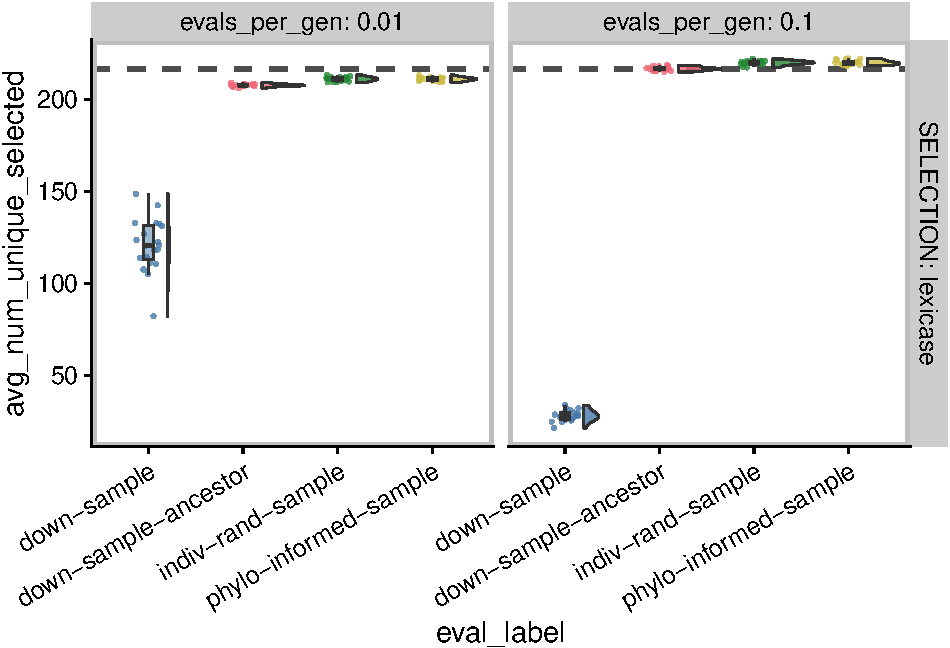
\includegraphics{phylogeny-informed-subsampling-supplemental_files/figure-latex/unnamed-chunk-17-1.pdf}

Average number selected by standard lexicase?

\begin{lstlisting}[language=R]
mean(filter(
  ts_summary_data,
  SELECTION == "lexicase" &
  DIAGNOSTIC == "exploitation-rate" &
  evals_per_gen == "1"
)$avg_num_unique_selected)
\end{lstlisting}

\begin{lstlisting}
## [1] 216.6185
\end{lstlisting}

\begin{lstlisting}[language=R]
mean(filter(
  ts_summary_data,
  SELECTION == "lexicase" &
  DIAGNOSTIC == "exploitation-rate" &
  evals_per_gen == "0.1",
  eval_label == "down-sample"
)$avg_num_unique_selected)
\end{lstlisting}

\begin{lstlisting}
## [1] 28.099
\end{lstlisting}

\begin{lstlisting}[language=R]
mean(filter(
  ts_summary_data,
  SELECTION == "lexicase" &
  DIAGNOSTIC == "exploitation-rate" &
  evals_per_gen == "0.01",
  eval_label == "down-sample"
)$avg_num_unique_selected)
\end{lstlisting}

\begin{lstlisting}
## [1] 120.7455
\end{lstlisting}

\hypertarget{manuscript-figures}{%
\section{Manuscript figures}\label{manuscript-figures}}

Figures customized / cleaned up for the manuscript.

\begin{lstlisting}[language=R]
build_final_score_manuscript_plot <- function(
  selection,
  subsample_rate
) {
  # Extract median values for max aggregate score at same evaluation level
  # as sampling regimes
  max_eval <- max(
    filter(exploit_ts_data, evals_per_gen == subsample_rate)$evaluations
  )
  full_eval_steps <- as.numeric(
    levels(
      as.factor(
        filter(exploit_ts_data, eval_label == "full" & evaluations >= max_eval)$evaluations # nolint: line_length_linter.
      )
    )
  )
  full_eval <- full_eval_steps[which.min( full_eval_steps  - max_eval )]
  full_median_score_evals <- median(
    filter(
      exploit_ts_data,
      SELECTION == selection & eval_label == "full" & evaluations == full_eval
    )$max_agg_score
  )

  plot <- exploit_summary_data %>%
    filter(
      eval_label != "full" &
      SELECTION == selection &
      evals_per_gen == subsample_rate
    ) %>%
    ggplot(
      aes(
        x = eval_label,
        y = elite_true_agg_score,
        fill = eval_label
      )
    ) +
    geom_hline(
      yintercept = full_median_score_evals,
      size = 1.0,
      alpha = 0.7,
      color = "black",
      linetype="dashed"
    ) +
    geom_flat_violin(
      position = position_nudge(x = .2, y = 0),
      alpha = .8,
      adjust = 1.5
    ) +
    geom_point(
      mapping = aes(color = eval_label),
      position = position_jitter(width = .15),
      size = .5,
      alpha = 0.8
    ) +
    geom_boxplot(
      width = .1,
      outlier.shape = NA,
      alpha = 0.5
    ) +
    scale_y_continuous(
      name = "Aggregate score",
      limits = c(0, 10010)
    ) +
    scale_x_discrete(
      name = "Subsampling regimes",
      breaks = c("down-sample", "down-sample-ancestor", "indiv-rand-sample", "phylo-informed-sample"),
      labels = c("DS", "DS+EST", "IRS", "ABS")
    ) +
    scale_fill_bright() +
    scale_color_bright() +
    theme(
      legend.position = "none",
      # axis.text.x = element_text(
      #   angle = 30,
      #   hjust = 1
      # ),
    )
  return(plot)
}
\end{lstlisting}

Build time series manuscript plot:

\begin{lstlisting}[language=R]
build_score_over_time_manuscript_plot <- function(
  selection,
  subsample_rate
) {

  max_eval <- max(
    filter(exploit_ts_data, evals_per_gen == subsample_rate)$evaluations
  )
  full_eval_steps <- as.numeric(
    levels(
      as.factor(
        filter(exploit_ts_data, eval_label == "full" & evaluations >= max_eval)$evaluations # nolint: line_length_linter.
      )
    )
  )
  full_eval <- full_eval_steps[which.min( full_eval_steps  - max_eval )]

  data <- exploit_ts_data %>%
    filter(
      SELECTION == selection &
      evals_per_gen == subsample_rate
    ) %>%
    mutate(
      sampling_level_label = subsample_rate
    )

  full_diag_data <- exploit_ts_data %>%
    filter(
      SELECTION == selection & eval_label == "full" & evaluations <= full_eval
    ) %>%
    mutate(
      # Ensure that median line will sit in same facet
      sampling_level_label = subsample_rate
    )

  plot <- data %>%
    filter(
      eval_label != "full"
    ) %>%
    ggplot(
      aes(
        x = evaluations,
        y = max_agg_score
      )
    ) +
    stat_summary(
      geom = "line",
      fun = mean,
      aes(
        color = eval_label
      )
    ) +
    stat_summary(
      geom = "ribbon",
      fun.data = "mean_cl_boot",
      fun.args = list(conf.int = 0.95),
      alpha = 0.2,
      linetype = 0,
      aes(
        color = eval_label,
        fill = eval_label
      )
    ) +
    scale_y_continuous(
      name = "Aggregate score",
      limits = c(0, 10010)
    ) +
    scale_x_continuous(
      name = "Evaluations"
    ) +
    scale_fill_bright(
      labels=c(
        "Down-sampling (DS), no estimation",
        "Down-sampling + Estimation (DS+EST)",
        "Individualized random sampling (IRS)",
        "Ancestor-based sampling (ABS)"
      )
    ) +
    scale_color_bright(
      labels=c(
        "Down-sampling (DS), no estimation",
        "Down-sampling + Estimation (DS+EST)",
        "Individualized random sampling (IRS)",
        "Ancestor-based sampling (ABS)"
      )
    ) +
    theme(
      legend.position = "none"
    ) +
    stat_summary(
      data = full_diag_data,
      geom = "line",
      fun = median,
      linetype = "dashed",
      color = "black"
    )

  return(plot)
}
\end{lstlisting}

Build plots of final scores (after fixed number of evaluations)

\begin{lstlisting}[language=R]
plot_final_lex_01 <- build_final_score_manuscript_plot(
  "lexicase",
  "0.01"
)
plot_final_lex_10 <- build_final_score_manuscript_plot(
  "lexicase",
  "0.1"
)
plot_final_tourn_01 <- build_final_score_manuscript_plot(
  "tournament",
  "0.01"
)
plot_final_tourn_10 <- build_final_score_manuscript_plot(
  "tournament",
  "0.1"
)
\end{lstlisting}

Build time series plots (with evaluations on x-axis)

\begin{lstlisting}[language=R]
plot_ts_lex_01 <- build_score_over_time_manuscript_plot(
  "lexicase",
  "0.01"
)

plot_ts_lex_10 <- build_score_over_time_manuscript_plot(
  "lexicase",
  "0.1"
)

plot_ts_tourn_01 <- build_score_over_time_manuscript_plot(
  "tournament",
  "0.01"
)

plot_ts_tourn_10 <- build_score_over_time_manuscript_plot(
  "tournament",
  "0.1"
)
\end{lstlisting}

\hypertarget{lexicase-selection-manuscript-figure}{%
\subsection{Lexicase selection manuscript figure}\label{lexicase-selection-manuscript-figure}}

\begin{lstlisting}[language=R]
txt_size <- 16
legend <- get_legend(
  plot_ts_lex_01 +
    guides(
      color = guide_legend(nrow = 2, title = "Subsampling regime:"),
      fill = guide_legend(nrow = 2, title = "Subsampling regime:")
    ) +
    theme(
      legend.position = "bottom",
      legend.text = element_text(size = txt_size - 2),
      legend.title = element_text(size = txt_size)
    )
)

grid <- plot_grid(
  plot_ts_lex_01 +
    labs(title = "1% Subsampling") +
    theme(
      axis.text.x = element_text(size = txt_size-2),
      axis.text.y = element_text(size = txt_size),
      axis.title.x = element_text(size = txt_size),
      axis.title.y = element_text(size = txt_size)
    ),
  plot_final_lex_01 +
    theme(
      axis.text.y = element_blank(),
      axis.title.y = element_blank(),
      axis.ticks.y = element_blank(),
      plot.margin = margin(0, 0, 0, 1, "cm"),
      axis.text.x = element_text(size = txt_size),
      axis.title.x = element_text(size = txt_size)
    ),
  plot_ts_lex_10 +
    labs(title = "10% Subsampling") +
    theme(
      axis.text.x = element_text(size = txt_size-2),
      axis.text.y = element_text(size = txt_size),
      axis.title.x = element_text(size = txt_size),
      axis.title.y = element_text(size = txt_size)
    ),
  plot_final_lex_10 +
    theme(
      axis.text.y = element_blank(),
      axis.title.y = element_blank(),
      axis.ticks.y = element_blank(),
      plot.margin = margin(0, 0, 0, 1, "cm"),
      axis.text.x = element_text(size = txt_size),
      axis.title.x = element_text(size = txt_size)
    ),
  nrow = 2,
  ncol = 2,
  align = "h",
  labels = c("a", "b", "c", "d"),
  label_size = 18,
  rel_widths = c(1.3, 1, 1.3, 1)
)

grid
\end{lstlisting}

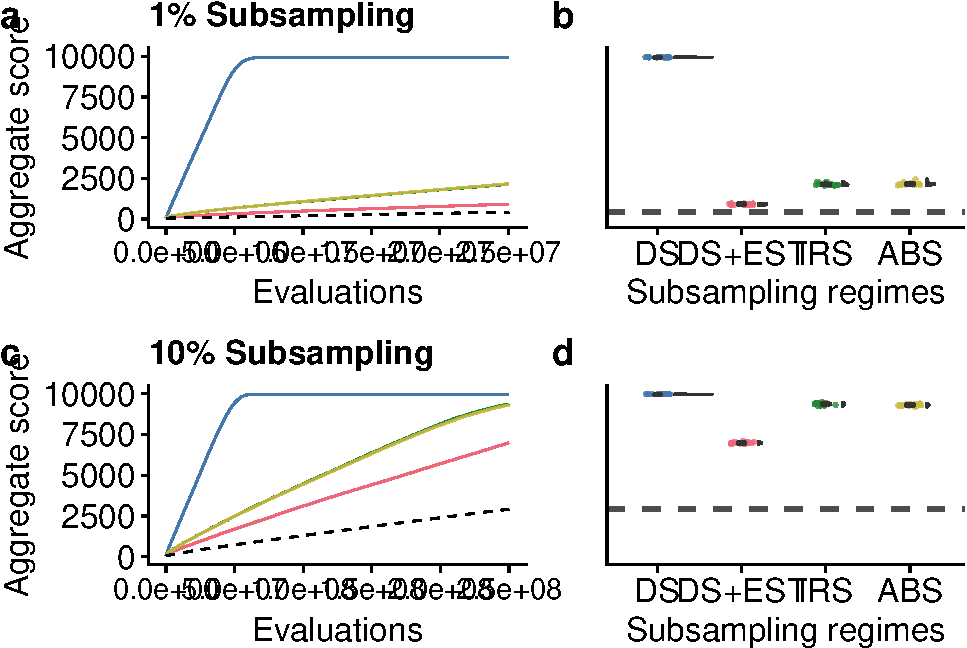
\includegraphics{phylogeny-informed-subsampling-supplemental_files/figure-latex/unnamed-chunk-24-1.pdf}

\begin{lstlisting}[language=R]
lex_fig <- plot_grid(
  grid,
  legend,
  nrow = 2,
  ncol = 1,
  rel_heights = c(1, 0.05)
)

# lex_fig
save_plot(
  filename = paste0(plot_directory, "2023-12-28-exploit-lex-fig.pdf"),
  plot = lex_fig,
  base_width = 10,
  base_height = 8,
  dpi = 600
)
\end{lstlisting}

\hypertarget{tournament-selection-manuscript-figures}{%
\subsection{Tournament selection manuscript figures}\label{tournament-selection-manuscript-figures}}

\begin{lstlisting}[language=R]
legend <- get_legend(
  plot_ts_tourn_01 +
    guides(
      color = guide_legend(nrow = 2, title = "Subsampling regime:"),
      fill = guide_legend(nrow = 2, title = "Subsampling regime:")
    ) +
    theme(
      legend.position = "bottom",
      legend.text = element_text(size = txt_size - 2),
      legend.title = element_text(size = txt_size)
    )
)

grid <- plot_grid(
  plot_ts_tourn_01 +
    labs(title = "1% Subsampling") +
    theme(
      axis.text.x = element_text(size = txt_size-2),
      axis.text.y = element_text(size = txt_size),
      axis.title.x = element_text(size = txt_size),
      axis.title.y = element_text(size = txt_size)
    ),
  plot_final_tourn_01 +
    theme(
      axis.text.y = element_blank(),
      axis.title.y = element_blank(),
      axis.ticks.y = element_blank(),
      plot.margin = margin(0, 0, 0, 1, "cm"),
      axis.text.x = element_text(size = txt_size),
      axis.title.x = element_text(size = txt_size)
    ),
  plot_ts_tourn_10 +
    labs(title = "10% Subsampling") +
    theme(
      axis.text.x = element_text(size = txt_size-2),
      axis.text.y = element_text(size = txt_size),
      axis.title.x = element_text(size = txt_size),
      axis.title.y = element_text(size = txt_size)
    ),
  plot_final_tourn_10 +
    theme(
      axis.text.y = element_blank(),
      axis.title.y = element_blank(),
      axis.ticks.y = element_blank(),
      plot.margin = margin(0, 0, 0, 1, "cm"),
      axis.text.x = element_text(size = txt_size),
      axis.title.x = element_text(size = txt_size)
    ),
  nrow = 2,
  ncol = 2,
  align = "h",
  labels = c("a", "b", "c", "d"),
  label_size = 18,
  rel_widths = c(1.3, 1, 1.3, 1)
)

tourn_fig <- plot_grid(
  grid,
  legend,
  nrow = 2,
  ncol = 1,
  rel_heights = c(1, 0.05)
)

tourn_fig
\end{lstlisting}

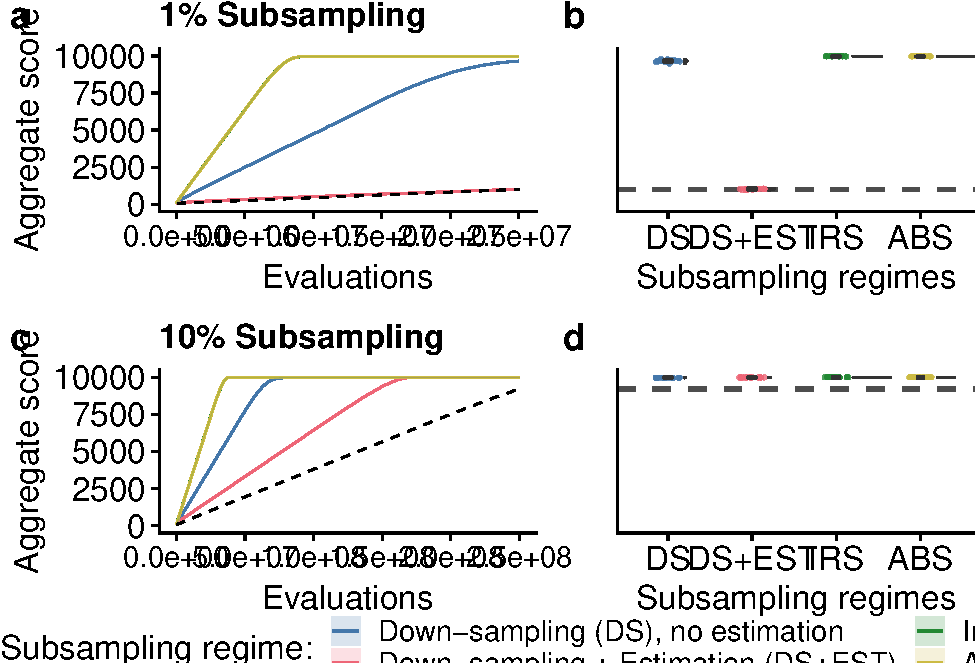
\includegraphics{phylogeny-informed-subsampling-supplemental_files/figure-latex/unnamed-chunk-25-1.pdf}

\begin{lstlisting}[language=R]
save_plot(
  filename = paste0(plot_directory, "2023-12-28-exploit-tourn-fig.pdf"),
  plot = tourn_fig,
  base_width = 10,
  base_height = 8,
  dpi = 600
)
\end{lstlisting}

\hypertarget{contradictory-objectives-diagnostic}{%
\chapter{Contradictory objectives diagnostic}\label{contradictory-objectives-diagnostic}}

\begin{lstlisting}[language=R]
experiment_slug <- "2023-12-28-phylo-sampling-diag"

working_directory <- paste0(
  "experiments/",
  experiment_slug,
  "/analysis/"
)

if (exists("bookdown_wd_prefix")) {
  working_directory <- paste0(
    bookdown_wd_prefix,
    working_directory
  )
}
\end{lstlisting}

\hypertarget{dependencies-1}{%
\section{Dependencies}\label{dependencies-1}}

\begin{lstlisting}[language=R]
library(tidyverse)
library(cowplot)
library(RColorBrewer)
library(khroma)
library(rstatix)
library(knitr)
source("https://gist.githubusercontent.com/benmarwick/2a1bb0133ff568cbe28d/raw/fb53bd97121f7f9ce947837ef1a4c65a73bffb3f/geom_flat_violin.R")
\end{lstlisting}

\begin{lstlisting}[language=R]
print(version)
\end{lstlisting}

\begin{lstlisting}
##                _                           
## platform       aarch64-apple-darwin20      
## arch           aarch64                     
## os             darwin20                    
## system         aarch64, darwin20           
## status                                     
## major          4                           
## minor          2.1                         
## year           2022                        
## month          06                          
## day            23                          
## svn rev        82513                       
## language       R                           
## version.string R version 4.2.1 (2022-06-23)
## nickname       Funny-Looking Kid
\end{lstlisting}

\hypertarget{setup-1}{%
\section{Setup}\label{setup-1}}

\begin{lstlisting}[language=R]
# Configure our default graphing theme
theme_set(theme_cowplot())
# Create a directory to store plots
plot_directory <- paste0(working_directory, "plots/")
dir.create(plot_directory, showWarnings=FALSE)
# Constants
focal_diagnostic <- "contradictory-objectives"
\end{lstlisting}

\hypertarget{load-experiment-summary-data-1}{%
\subsection{Load experiment summary data}\label{load-experiment-summary-data-1}}

\begin{lstlisting}[language=R]
summary_data_loc <- paste0(working_directory, "data/aggregate.csv")
summary_data <- read_csv(summary_data_loc)
\end{lstlisting}

\begin{lstlisting}
## Rows: 1080 Columns: 58
## -- Column specification -----------------------------------------------------------------------------------------------------------------------------------------------------------------------------------------
## Delimiter: ","
## chr  (5): DIAGNOSTIC, EVAL_FIT_EST_MODE, EVAL_MODE, SELECTION, STOP_MODE
## dbl (53): ACCURACY, CREDIT, DIAGNOSTIC_DIMENSIONALITY, EVAL_MAX_PHYLO_SEARCH...
## 
## i Use `spec()` to retrieve the full column specification for this data.
## i Specify the column types or set `show_col_types = FALSE` to quiet this message.
\end{lstlisting}

\begin{lstlisting}[language=R]
summary_data <- summary_data %>%
  mutate(
    evals_per_gen = case_when(
      EVAL_MODE == "cohort-full-compete" ~ 1.0 / NUM_COHORTS,
      EVAL_MODE == "cohort" ~ 1.0 / NUM_COHORTS,
      EVAL_MODE == "down-sample" ~ TEST_DOWNSAMPLE_RATE,
      EVAL_MODE == "full" ~ 1.0,
      EVAL_MODE == "indiv-rand-sample" ~ TEST_DOWNSAMPLE_RATE,
      EVAL_MODE == "phylo-informed-sample" ~ TEST_DOWNSAMPLE_RATE
    ),
    EVAL_FIT_EST_MODE = case_when(
      EVAL_FIT_EST_MODE == "ancestor-opt" ~ "ancestor",
      EVAL_FIT_EST_MODE == "relative-opt" ~ "relative",
      .default = EVAL_FIT_EST_MODE
    ),
    .keep = "all"
  ) %>%
  mutate(
    eval_label = case_when(
      # Clean up down-sample label
      EVAL_MODE == "down-sample" & EVAL_FIT_EST_MODE != "none" ~ paste("down-sample", EVAL_FIT_EST_MODE, sep="-"),
      .default = EVAL_MODE
    ),
  ) %>%
  mutate(
    evals_per_gen = as.factor(evals_per_gen),
    DIAGNOSTIC = as.factor(DIAGNOSTIC),
    SELECTION = as.factor(SELECTION),
    EVAL_MODE = as.factor(EVAL_MODE),
    NUM_COHORTS = as.factor(NUM_COHORTS),
    TEST_DOWNSAMPLE_RATE = as.factor(TEST_DOWNSAMPLE_RATE),
    EVAL_FIT_EST_MODE = factor(
      EVAL_FIT_EST_MODE,
      levels = c(
        "none",
        "ancestor",
        "relative"
      ),
      labels = c(
        "None",
        "Ancestor",
        "Relative"
      )
    )
  )

# Grab just the contradictory objectives data
con_obj_summary_data <- filter(
  summary_data,
  DIAGNOSTIC == "contradictory-objectives"
)
\end{lstlisting}

\hypertarget{load-experiment-time-series-data-1}{%
\subsection{Load experiment time series data}\label{load-experiment-time-series-data-1}}

\begin{lstlisting}[language=R]
ts_data_loc <- paste0(working_directory, "data/time_series.csv")
ts_data <- read_csv(ts_data_loc)
\end{lstlisting}

\begin{lstlisting}
## Rows: 108000 Columns: 28
## -- Column specification -----------------------------------------------------------------------------------------------------------------------------------------------------------------------------------------
## Delimiter: ","
## chr  (4): DIAGNOSTIC, EVAL_FIT_EST_MODE, EVAL_MODE, SELECTION
## dbl (24): NUM_COHORTS, SEED, TEST_DOWNSAMPLE_RATE, ave_depth, deleterious_st...
## 
## i Use `spec()` to retrieve the full column specification for this data.
## i Specify the column types or set `show_col_types = FALSE` to quiet this message.
\end{lstlisting}

\begin{lstlisting}[language=R]
ts_data <- ts_data %>%
  mutate(
    evals_per_gen = case_when(
      EVAL_MODE == "cohort-full-compete" ~ 1.0 / NUM_COHORTS,
      EVAL_MODE == "cohort" ~ 1.0 / NUM_COHORTS,
      EVAL_MODE == "down-sample" ~ TEST_DOWNSAMPLE_RATE,
      EVAL_MODE == "full" ~ 1.0,
      EVAL_MODE == "indiv-rand-sample" ~ TEST_DOWNSAMPLE_RATE,
      EVAL_MODE == "phylo-informed-sample" ~ TEST_DOWNSAMPLE_RATE
    ),
    EVAL_FIT_EST_MODE = case_when(
      EVAL_FIT_EST_MODE == "ancestor-opt" ~ "ancestor",
      EVAL_FIT_EST_MODE == "relative-opt" ~ "relative",
      .default = EVAL_FIT_EST_MODE
    ),
    .keep = "all"
  ) %>%
  mutate(
    eval_label = case_when(
      EVAL_MODE == "down-sample" & EVAL_FIT_EST_MODE != "none" ~ paste("down-sample", EVAL_FIT_EST_MODE, sep="-"),
      .default = EVAL_MODE
    )
  ) %>%
  mutate(
    evals_per_gen = as.factor(evals_per_gen),
    DIAGNOSTIC = as.factor(DIAGNOSTIC),
    SELECTION = as.factor(SELECTION),
    EVAL_MODE = as.factor(EVAL_MODE),
    NUM_COHORTS = as.factor(NUM_COHORTS),
    TEST_DOWNSAMPLE_RATE = as.factor(TEST_DOWNSAMPLE_RATE),
    EVAL_FIT_EST_MODE = factor(
      EVAL_FIT_EST_MODE,
      levels = c(
        "none",
        "ancestor",
        "relative"
      ),
      labels = c(
        "None",
        "Ancestor",
        "Relative"
      )
    )
  )

# Grab just the contradictory objectives data
con_obj_ts_data <- ts_data %>%
  filter(DIAGNOSTIC == "contradictory-objectives")
\end{lstlisting}

Summarize time series data:

\begin{lstlisting}[language=R]
ts_summary_data <- ts_data %>%
  group_by(SEED, DIAGNOSTIC, SELECTION, evals_per_gen, eval_label) %>%
  summarize(
    n = n(),
    avg_num_unique_selected = mean(num_unique_selected),
    total_optimal_trait_coverage_loss = sum(optimal_trait_coverage_loss)
  )
\end{lstlisting}

\begin{lstlisting}
## `summarise()` has grouped output by 'SEED', 'DIAGNOSTIC', 'SELECTION',
## 'evals_per_gen'. You can override using the `.groups` argument.
\end{lstlisting}

\hypertarget{plotting-helper-functions-1}{%
\subsection{Plotting helper functions}\label{plotting-helper-functions-1}}

The following function assist with exploratory plotting of different measurements from summary and time series data.
Note that for these plots, standard lexicase reference is rendered at equivalent number of generations (instead of evaluations).

\begin{lstlisting}[language=R]
build_plot_summary_data <- function(data, diagnostic, selection, response) {
  diag_data <- data %>% filter(DIAGNOSTIC == diagnostic)

  full_median <- median(
    filter(
      diag_data,
      eval_label == "full" & SELECTION == selection
    )[[response]]
  )

  plot <- diag_data %>%
    filter(
      eval_label != "full" & SELECTION == selection
    ) %>%
    ggplot(
      aes_string(
        x = "eval_label",
        y = response,
        fill = "eval_label"
      )
    ) +
    geom_hline(
      yintercept = full_median,
      size = 1.0,
      alpha = 0.7,
      color = "black",
      linetype="dashed"
    ) +
    geom_flat_violin(
      position = position_nudge(x = .2, y = 0),
      alpha = .8,
      adjust = 1.5
    ) +
    geom_point(
      mapping = aes(color = eval_label),
      position = position_jitter(width = .15),
      size = .5,
      alpha = 0.8
    ) +
    geom_boxplot(
      width = .1,
      outlier.shape = NA,
      alpha = 0.5
    ) +
    scale_y_continuous(
      # limits = c(-0.5, 100)
    ) +
    scale_fill_bright() +
    scale_color_bright() +
    facet_grid(
      SELECTION ~ evals_per_gen,
      # nrow=2,
      labeller = label_both
    ) +
    theme(
      legend.position = "none",
      axis.text.x = element_text(
        angle = 30,
        hjust = 1
      ),
      panel.border = element_rect(color = "gray", size = 2)
    )

  return(plot)
}

build_plot_time_series_single_sampling <- function(
  data,
  diagnostic,
  selection,
  sampling_level,
  response
) {

  diag_data <- data %>% filter(
    DIAGNOSTIC == diagnostic &
    SELECTION == selection &
    evals_per_gen == sampling_level
  ) %>%
  mutate(
    sampling_level_label = sampling_level
  )

  full_diag_data <- data %>% filter(
    DIAGNOSTIC == diagnostic & SELECTION == selection & eval_label == "full"
  ) %>%
  mutate(
    # Ensure that median line will sit in same facet
    sampling_level_label = sampling_level
  )

  plot <- diag_data %>%
    filter(
      eval_label != "full"
    ) %>%
    ggplot(
      aes_string(
        x = "ts_step",
        # x = "evaluations",
        y = {{ response }}
      )
    ) +
    stat_summary(
      geom = "line",
      fun = mean,
      aes(
        color = eval_label
      )
    ) +
    stat_summary(
      geom = "ribbon",
      fun.data = "mean_cl_boot",
      fun.args = list(conf.int = 0.95),
      alpha = 0.2,
      linetype = 0,
      aes(
        color = eval_label,
        fill = eval_label
      )
    ) +
    scale_fill_bright() +
    scale_color_bright() +
    # facet_wrap(
    #   ~ sampling_level_label,
    #   ncol = 1,
    #   labeller = label_both
    # ) +
    theme(
      legend.position = "right"
    ) +
    stat_summary(
      data = full_diag_data,
      geom = "line",
      fun = median,
      linetype = "dashed",
      color = "black"
    )

  return(plot)
}

build_plot_time_series <- function(
  data,
  diagnostic,
  selection,
  response
) {
  # Build 1% sampling plot and 10% sampling plot
  p_01 <- data  %>% build_plot_time_series_single_sampling(
    diagnostic,
    selection,
    "0.01",
    response
  )
  p_10 <- data %>% build_plot_time_series_single_sampling(
    diagnostic,
    selection,
    "0.1",
    response
  )

  title <- ggdraw() +
    draw_label(
      paste0(diagnostic, " - ", selection),
      fontface = 'bold',
      x = 0,
      hjust = 0
    ) +
    theme(
      # add margin on the left of the drawing canvas,
      # so title is aligned with left edge of first plot
      plot.margin = margin(0, 0, 0, 7)
    )

  plot <- plot_grid(
    title,
    p_01 + labs(title = "1% subsampling") + theme(legend.position = "none"),
    p_10 + labs(title = "10% subsampling") + theme(legend.position = "bottom"),
    nrow = 3,
    ncol = 1,
    rel_heights = c(0.075, 1, 1)
  )

  return(plot)
}
\end{lstlisting}

\hypertarget{population-wide-satisfactory-trait-coverage}{%
\section{Population-wide satisfactory trait coverage}\label{population-wide-satisfactory-trait-coverage}}

\hypertarget{final---lexicase-selection-1}{%
\subsection{Final - Lexicase selection}\label{final---lexicase-selection-1}}

\begin{lstlisting}[language=R]
p <- summary_data %>% build_plot_summary_data(
  focal_diagnostic,
  "lexicase",
  "pop_optimal_trait_coverage"
)
ggsave(
  filename = paste0(plot_directory, "con-obj-sat-cov-final-lex.pdf"),
  plot = p + labs(title = "Contradictory objectives - Lexicase selection"),
  width = 15,
  height = 10
)
\end{lstlisting}

\hypertarget{statistics}{%
\subsubsection{Statistics}\label{statistics}}

First, we'll create a table of median / mean values for easy reference.

\begin{lstlisting}[language=R]
con_obj_summary_data %>%
  group_by(DIAGNOSTIC, SELECTION, evals_per_gen, eval_label) %>%
  summarize(
    cov_median = median(pop_optimal_trait_coverage),
    cov_mean = mean(pop_optimal_trait_coverage),
    replicates = n()
  ) %>%
  kable()
\end{lstlisting}

\begin{lstlisting}
## `summarise()` has grouped output by 'DIAGNOSTIC', 'SELECTION', 'evals_per_gen'.
## You can override using the `.groups` argument.
\end{lstlisting}

\begin{tabular}{l|l|l|l|r|r|r}
\hline
DIAGNOSTIC & SELECTION & evals\_per\_gen & eval\_label & cov\_median & cov\_mean & replicates\\
\hline
contradictory-objectives & lexicase & 0.01 & down-sample & 1.0 & 1.00 & 20\\
\hline
contradictory-objectives & lexicase & 0.01 & down-sample-ancestor & 2.5 & 3.25 & 20\\
\hline
contradictory-objectives & lexicase & 0.01 & indiv-rand-sample & 8.0 & 8.20 & 20\\
\hline
contradictory-objectives & lexicase & 0.01 & phylo-informed-sample & 8.5 & 8.90 & 20\\
\hline
contradictory-objectives & lexicase & 0.1 & down-sample & 1.0 & 1.00 & 20\\
\hline
contradictory-objectives & lexicase & 0.1 & down-sample-ancestor & 17.5 & 18.15 & 20\\
\hline
contradictory-objectives & lexicase & 0.1 & indiv-rand-sample & 24.5 & 24.10 & 20\\
\hline
contradictory-objectives & lexicase & 0.1 & phylo-informed-sample & 24.0 & 24.25 & 20\\
\hline
contradictory-objectives & lexicase & 1 & full & 38.0 & 37.85 & 20\\
\hline
contradictory-objectives & tournament & 0.01 & down-sample & 1.0 & 1.00 & 20\\
\hline
contradictory-objectives & tournament & 0.01 & down-sample-ancestor & 1.0 & 1.00 & 20\\
\hline
contradictory-objectives & tournament & 0.01 & indiv-rand-sample & 1.0 & 1.00 & 20\\
\hline
contradictory-objectives & tournament & 0.01 & phylo-informed-sample & 1.0 & 1.00 & 20\\
\hline
contradictory-objectives & tournament & 0.1 & down-sample & 1.0 & 1.00 & 20\\
\hline
contradictory-objectives & tournament & 0.1 & down-sample-ancestor & 1.0 & 1.00 & 20\\
\hline
contradictory-objectives & tournament & 0.1 & indiv-rand-sample & 1.0 & 1.00 & 20\\
\hline
contradictory-objectives & tournament & 0.1 & phylo-informed-sample & 1.0 & 1.00 & 20\\
\hline
contradictory-objectives & tournament & 1 & full & 1.0 & 1.00 & 20\\
\hline
\end{tabular}

Next, we run a Kruskal-Wallis test to check for differences.
For these tests, we only compare within a single subsampling level (\passthrough{\lstinline!evals\_per\_gen!}) and within the same selection scheme.

\begin{lstlisting}[language=R]
kw_test <- con_obj_summary_data %>%
  filter(eval_label != "full") %>%
  group_by(SELECTION, evals_per_gen) %>%
  kruskal_test(pop_optimal_trait_coverage ~ eval_label) %>%
  mutate(sig = (p < 0.05)) %>%
  unite(
    "comparison_group",
    SELECTION,
    evals_per_gen,
    sep = "_",
    remove = FALSE
  )
kable(kw_test)
\end{lstlisting}

\begin{tabular}{l|l|l|l|r|r|r|r|l|l}
\hline
comparison\_group & SELECTION & evals\_per\_gen & .y. & n & statistic & df & p & method & sig\\
\hline
lexicase\_0.01 & lexicase & 0.01 & pop\_optimal\_trait\_coverage & 80 & 58.24682 & 3 & 0 & Kruskal-Wallis & TRUE\\
\hline
lexicase\_0.1 & lexicase & 0.1 & pop\_optimal\_trait\_coverage & 80 & 62.11510 & 3 & 0 & Kruskal-Wallis & TRUE\\
\hline
tournament\_0.01 & tournament & 0.01 & pop\_optimal\_trait\_coverage & 80 & NaN & 3 & NaN & Kruskal-Wallis & NA\\
\hline
tournament\_0.1 & tournament & 0.1 & pop\_optimal\_trait\_coverage & 80 & NaN & 3 & NaN & Kruskal-Wallis & NA\\
\hline
\end{tabular}

\begin{lstlisting}[language=R]
# Grab group names of significant comparisons
sig_kw_groups <- filter(kw_test, p < 0.05)$comparison_group

wrs_test <- con_obj_summary_data %>%
  unite(
    "comparison_group",
    SELECTION,
    evals_per_gen,
    sep = "_",
    remove = FALSE
  ) %>%
  filter(
    eval_label != "full" & comparison_group %in% sig_kw_groups
  ) %>%
  group_by(SELECTION, evals_per_gen) %>%
  pairwise_wilcox_test(pop_optimal_trait_coverage ~ eval_label) %>%
  adjust_pvalue(method = "holm") %>%
  add_significance("p.adj")

kable(wrs_test)
\end{lstlisting}

\begin{tabular}{l|l|l|l|l|r|r|r|r|r|l}
\hline
SELECTION & evals\_per\_gen & .y. & group1 & group2 & n1 & n2 & statistic & p & p.adj & p.adj.signif\\
\hline
lexicase & 0.01 & pop\_optimal\_trait\_coverage & down-sample & down-sample-ancestor & 20 & 20 & 50 & 3.20e-06 & 1.91e-05 & ****\\
\hline
lexicase & 0.01 & pop\_optimal\_trait\_coverage & down-sample & indiv-rand-sample & 20 & 20 & 0 & 0.00e+00 & 1.00e-07 & ****\\
\hline
lexicase & 0.01 & pop\_optimal\_trait\_coverage & down-sample & phylo-informed-sample & 20 & 20 & 0 & 0.00e+00 & 1.00e-07 & ****\\
\hline
lexicase & 0.01 & pop\_optimal\_trait\_coverage & down-sample-ancestor & indiv-rand-sample & 20 & 20 & 37 & 9.80e-06 & 2.93e-05 & ****\\
\hline
lexicase & 0.01 & pop\_optimal\_trait\_coverage & down-sample-ancestor & phylo-informed-sample & 20 & 20 & 28 & 3.20e-06 & 1.91e-05 & ****\\
\hline
lexicase & 0.01 & pop\_optimal\_trait\_coverage & indiv-rand-sample & phylo-informed-sample & 20 & 20 & 181 & 6.14e-01 & 1.00e+00 & ns\\
\hline
lexicase & 0.1 & pop\_optimal\_trait\_coverage & down-sample & down-sample-ancestor & 20 & 20 & 0 & 0.00e+00 & 1.00e-07 & ****\\
\hline
lexicase & 0.1 & pop\_optimal\_trait\_coverage & down-sample & indiv-rand-sample & 20 & 20 & 0 & 0.00e+00 & 1.00e-07 & ****\\
\hline
lexicase & 0.1 & pop\_optimal\_trait\_coverage & down-sample & phylo-informed-sample & 20 & 20 & 0 & 0.00e+00 & 1.00e-07 & ****\\
\hline
lexicase & 0.1 & pop\_optimal\_trait\_coverage & down-sample-ancestor & indiv-rand-sample & 20 & 20 & 31 & 4.90e-06 & 1.95e-05 & ****\\
\hline
lexicase & 0.1 & pop\_optimal\_trait\_coverage & down-sample-ancestor & phylo-informed-sample & 20 & 20 & 24 & 1.90e-06 & 1.32e-05 & ****\\
\hline
lexicase & 0.1 & pop\_optimal\_trait\_coverage & indiv-rand-sample & phylo-informed-sample & 20 & 20 & 203 & 9.46e-01 & 1.00e+00 & ns\\
\hline
\end{tabular}

\hypertarget{over-time---lexicase-selection}{%
\subsection{Over time - lexicase selection}\label{over-time---lexicase-selection}}

\begin{lstlisting}[language=R]
p <- ts_data  %>% build_plot_time_series(
  focal_diagnostic,
  "lexicase",
  "pop_optimal_trait_coverage"
)
ggsave(
  filename = paste0(plot_directory, "con-obj-sat-cov-ts-lex.pdf"),
  plot = p,
  width = 15,
  height = 10
)
\end{lstlisting}

\hypertarget{final---tournament-selection-1}{%
\subsection{Final - Tournament selection}\label{final---tournament-selection-1}}

\begin{lstlisting}[language=R]
p <- summary_data %>% build_plot_summary_data(
  focal_diagnostic,
  "tournament",
  "pop_optimal_trait_coverage"
)
ggsave(
  filename = paste0(plot_directory, "con-obj-sat-cov-final-tourn.pdf"),
  plot = p + labs(title = "Contradictory objectives - Tournament selection"),
  width = 15,
  height = 10
)
\end{lstlisting}

\hypertarget{over-time---tournament-selection}{%
\subsection{Over time - tournament selection}\label{over-time---tournament-selection}}

\begin{lstlisting}[language=R]
p <- ts_data  %>% build_plot_time_series(
  focal_diagnostic,
  "tournament",
  "pop_optimal_trait_coverage"
)
ggsave(
  filename = paste0(plot_directory, "con-obj-sat-cov-ts-tourn.pdf"),
  plot = p,
  width = 15,
  height = 10
)
\end{lstlisting}

\hypertarget{mrca-changes}{%
\section{MRCA changes}\label{mrca-changes}}

\begin{lstlisting}[language=R]
p <- summary_data %>% build_plot_summary_data(
  focal_diagnostic,
  "lexicase",
  "phylo_mrca_changes"
)
ggsave(
  filename = paste0(plot_directory, "con-obj-mrca-chgs-final-lex.pdf"),
  plot = p + labs(title = "Contradictory objectives - Lexicase selection"),
  width = 15,
  height = 10
)
\end{lstlisting}

\hypertarget{mean-genotype-deleterious-steps}{%
\section{Mean genotype deleterious steps}\label{mean-genotype-deleterious-steps}}

\begin{lstlisting}[language=R]
p <- summary_data %>% build_plot_summary_data(
  focal_diagnostic,
  "lexicase",
  "phylo_mean_genoetype_deleterious_steps"
)
ggsave(
  filename = paste0(plot_directory, "con-obj-del-steps-final-lex.pdf"),
  plot = p + labs(title = "Contradictory objectives - Lexicase selection"),
  width = 15,
  height = 10
)
\end{lstlisting}

\hypertarget{mean-genotype-pairwise-distance}{%
\section{Mean genotype pairwise distance}\label{mean-genotype-pairwise-distance}}

\begin{lstlisting}[language=R]
p <- summary_data %>% build_plot_summary_data(
  focal_diagnostic,
  "lexicase",
  "phylo_mean_genotype_pairwise_distance"
)
ggsave(
  filename = paste0(plot_directory, "con-obj-pw-dist-final-lex.pdf"),
  plot = p + labs(title = "Contradictory objectives - Lexicase selection"),
  width = 15,
  height = 10
)
\end{lstlisting}

\hypertarget{number-unique-individual-selected-1}{%
\section{Number unique individual selected}\label{number-unique-individual-selected-1}}

\begin{lstlisting}[language=R]
build_plot_summary_data(
  ts_summary_data,
  focal_diagnostic,
  "lexicase",
  "avg_num_unique_selected"
)
\end{lstlisting}

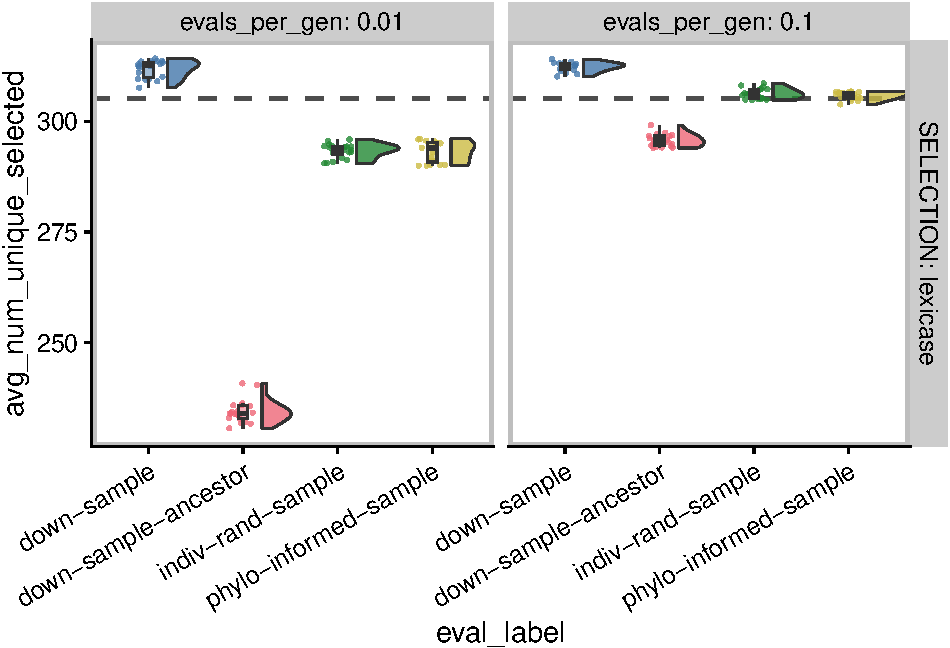
\includegraphics{phylogeny-informed-subsampling-supplemental_files/figure-latex/unnamed-chunk-45-1.pdf}

\hypertarget{manuscript-figures-1}{%
\section{Manuscript figures}\label{manuscript-figures-1}}

Time series graphs don't add a ton here, so just final graphs.

\begin{lstlisting}[language=R]
build_final_score_manuscript_plot <- function(
  selection,
  subsample_rate
) {

  # Extract median values for max aggregate score at same evaluation level as sampling regimes
  max_eval <- max(
    filter(con_obj_summary_data, evals_per_gen == subsample_rate)$evaluations
  )
  full_eval_steps <- as.numeric(
    levels(
      as.factor(
        filter(con_obj_summary_data, eval_label == "full" & evaluations >= max_eval)$evaluations # nolint: line_length_linter.
      )
    )
  )
  full_eval <- full_eval_steps[which.min( full_eval_steps  - max_eval )]
  full_median_score_evals <- median(
    filter(
      con_obj_summary_data,
      SELECTION == selection & eval_label == "full" & evaluations == full_eval
    )$pop_optimal_trait_coverage
  )

  plot <- con_obj_summary_data %>%
    filter(
      eval_label != "full" &
      SELECTION == selection &
      evals_per_gen == subsample_rate
    ) %>%
    ggplot(
      aes(
        x = eval_label,
        y = pop_optimal_trait_coverage,
        fill = eval_label
      )
    ) +
    geom_hline(
      yintercept = full_median_score_evals,
      size = 1.0,
      alpha = 0.7,
      color = "black",
      linetype="dashed"
    ) +
    geom_flat_violin(
      position = position_nudge(x = .2, y = 0),
      alpha = .8,
      adjust = 1.5
    ) +
    geom_point(
      mapping = aes(color = eval_label),
      position = position_jitter(width = .15),
      size = .5,
      alpha = 0.8
    ) +
    geom_boxplot(
      width = .1,
      outlier.shape = NA,
      alpha = 0.5
    ) +
    scale_y_continuous(
      name = "Satisfactory trait coverage",
      limits = c(0, 100)
    ) +
    scale_x_discrete(
      name = "Subsampling regime",
      breaks = c("down-sample", "down-sample-ancestor", "indiv-rand-sample", "phylo-informed-sample"),
      labels = c("DS\n(no est.)", "DS+EST", "IRS", "ABS")
    ) +
    scale_fill_bright() +
    scale_color_bright() +
    theme(
      legend.position = "none",
      # axis.text.x = element_text(
      #   angle = 30,
      #   hjust = 1
      # ),
    )
  return(plot)
}
\end{lstlisting}

Build end-of-run plots (fixed number of evaluations)

\begin{lstlisting}[language=R]
plot_final_lex_01 <- build_final_score_manuscript_plot(
  "lexicase",
  "0.01"
)
plot_final_lex_10 <- build_final_score_manuscript_plot(
  "lexicase",
  "0.1"
)
\end{lstlisting}

Combine into single figure

\begin{lstlisting}[language=R]
lex_fig <- plot_grid(
  plot_final_lex_01 +
    # labs(
    #   title = "1% subsampling"
    # ) +
    theme(
      plot.margin = margin(1, 0, 0, 0, "cm")
    ),
  plot_final_lex_10 +
    # labs(
    #   title = "10% subsampling"
    # ) +
    theme(
      axis.text.y = element_blank(),
      axis.title.y = element_blank(),
      axis.ticks.y = element_blank(),
      plot.margin = margin(1, 0, 0, 1, "cm")
    ),
  nrow = 1,
  ncol = 2,
  align = "h",
  labels = c("a) 1% subsampling", "b) 10% subsampling"),
  rel_widths = c(1, 1)
)
lex_fig
\end{lstlisting}

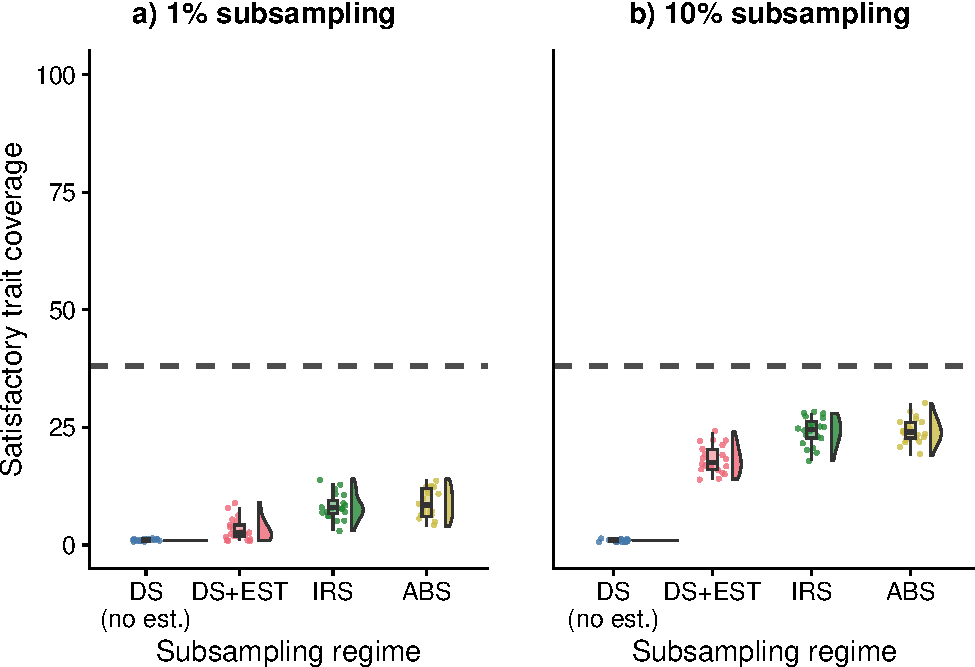
\includegraphics{phylogeny-informed-subsampling-supplemental_files/figure-latex/unnamed-chunk-48-1.pdf}

\begin{lstlisting}[language=R]
save_plot(
  filename = paste0(plot_directory, "2023-12-28-con-obj-lex-fig.pdf"),
  plot = lex_fig,
  base_width = 7,
  base_height = 4,
  dpi = 600
)
\end{lstlisting}

\hypertarget{multi-path-exploration-diagnostic}{%
\chapter{Multi-path exploration diagnostic}\label{multi-path-exploration-diagnostic}}

\begin{lstlisting}[language=R]
experiment_slug <- "2023-12-28-phylo-sampling-diag"

working_directory <- paste0(
  "experiments/",
  experiment_slug,
  "/analysis/"
)

if (exists("bookdown_wd_prefix")) {
  working_directory <- paste0(
    bookdown_wd_prefix,
    working_directory
  )
}
\end{lstlisting}

\hypertarget{dependencies-2}{%
\section{Dependencies}\label{dependencies-2}}

\begin{lstlisting}[language=R]
library(tidyverse)
library(cowplot)
library(RColorBrewer)
library(khroma)
library(rstatix)
library(knitr)
source("https://gist.githubusercontent.com/benmarwick/2a1bb0133ff568cbe28d/raw/fb53bd97121f7f9ce947837ef1a4c65a73bffb3f/geom_flat_violin.R")
\end{lstlisting}

\begin{lstlisting}[language=R]
print(version)
\end{lstlisting}

\begin{lstlisting}
##                _                           
## platform       aarch64-apple-darwin20      
## arch           aarch64                     
## os             darwin20                    
## system         aarch64, darwin20           
## status                                     
## major          4                           
## minor          2.1                         
## year           2022                        
## month          06                          
## day            23                          
## svn rev        82513                       
## language       R                           
## version.string R version 4.2.1 (2022-06-23)
## nickname       Funny-Looking Kid
\end{lstlisting}

\hypertarget{setup-2}{%
\section{Setup}\label{setup-2}}

\begin{lstlisting}[language=R]
# Configure our default graphing theme
theme_set(theme_cowplot())
# Create a directory to store plots
plot_directory <- paste0(working_directory, "plots/")
dir.create(plot_directory, showWarnings=FALSE)
# Constants
focal_diagnostic <- "multipath-exploration"
\end{lstlisting}

\hypertarget{load-experiment-summary-data-2}{%
\subsection{Load experiment summary data}\label{load-experiment-summary-data-2}}

\begin{lstlisting}[language=R]
summary_data_loc <- paste0(working_directory, "data/aggregate.csv")
summary_data <- read_csv(summary_data_loc)
\end{lstlisting}

\begin{lstlisting}
## Rows: 1080 Columns: 58
## -- Column specification -----------------------------------------------------------------------------------------------------------------------------------------------------------------------------------------
## Delimiter: ","
## chr  (5): DIAGNOSTIC, EVAL_FIT_EST_MODE, EVAL_MODE, SELECTION, STOP_MODE
## dbl (53): ACCURACY, CREDIT, DIAGNOSTIC_DIMENSIONALITY, EVAL_MAX_PHYLO_SEARCH...
## 
## i Use `spec()` to retrieve the full column specification for this data.
## i Specify the column types or set `show_col_types = FALSE` to quiet this message.
\end{lstlisting}

\begin{lstlisting}[language=R]
summary_data <- summary_data %>%
  mutate(
    evals_per_gen = case_when(
      EVAL_MODE == "cohort-full-compete" ~ 1.0 / NUM_COHORTS,
      EVAL_MODE == "cohort" ~ 1.0 / NUM_COHORTS,
      EVAL_MODE == "down-sample" ~ TEST_DOWNSAMPLE_RATE,
      EVAL_MODE == "full" ~ 1.0,
      EVAL_MODE == "indiv-rand-sample" ~ TEST_DOWNSAMPLE_RATE,
      EVAL_MODE == "phylo-informed-sample" ~ TEST_DOWNSAMPLE_RATE
    ),
    EVAL_FIT_EST_MODE = case_when(
      EVAL_FIT_EST_MODE == "ancestor-opt" ~ "ancestor",
      EVAL_FIT_EST_MODE == "relative-opt" ~ "relative",
      .default = EVAL_FIT_EST_MODE
    ),
    .keep = "all"
  ) %>%
  mutate(
    eval_label = case_when(
      # Clean up down-sample label
      EVAL_MODE == "down-sample" & EVAL_FIT_EST_MODE != "none" ~ paste("down-sample", EVAL_FIT_EST_MODE, sep="-"),
      .default = EVAL_MODE
    ),
  ) %>%
  mutate(
    evals_per_gen = as.factor(evals_per_gen),
    DIAGNOSTIC = as.factor(DIAGNOSTIC),
    SELECTION = as.factor(SELECTION),
    EVAL_MODE = as.factor(EVAL_MODE),
    NUM_COHORTS = as.factor(NUM_COHORTS),
    TEST_DOWNSAMPLE_RATE = as.factor(TEST_DOWNSAMPLE_RATE),
    EVAL_FIT_EST_MODE = factor(
      EVAL_FIT_EST_MODE,
      levels = c(
        "none",
        "ancestor",
        "relative"
      ),
      labels = c(
        "None",
        "Ancestor",
        "Relative"
      )
    )
  )

explore_summary_data <- filter(
  summary_data,
  DIAGNOSTIC == "multipath-exploration"
)
\end{lstlisting}

\hypertarget{load-experiment-time-series-data-2}{%
\subsection{Load experiment time series data}\label{load-experiment-time-series-data-2}}

\begin{lstlisting}[language=R]
ts_data_loc <- paste0(working_directory, "data/time_series.csv")
ts_data <- read_csv(ts_data_loc)
\end{lstlisting}

\begin{lstlisting}
## Rows: 108000 Columns: 28
## -- Column specification -----------------------------------------------------------------------------------------------------------------------------------------------------------------------------------------
## Delimiter: ","
## chr  (4): DIAGNOSTIC, EVAL_FIT_EST_MODE, EVAL_MODE, SELECTION
## dbl (24): NUM_COHORTS, SEED, TEST_DOWNSAMPLE_RATE, ave_depth, deleterious_st...
## 
## i Use `spec()` to retrieve the full column specification for this data.
## i Specify the column types or set `show_col_types = FALSE` to quiet this message.
\end{lstlisting}

\begin{lstlisting}[language=R]
ts_data <- ts_data %>%
  mutate(
    evals_per_gen = case_when(
      EVAL_MODE == "cohort-full-compete" ~ 1.0 / NUM_COHORTS,
      EVAL_MODE == "cohort" ~ 1.0 / NUM_COHORTS,
      EVAL_MODE == "down-sample" ~ TEST_DOWNSAMPLE_RATE,
      EVAL_MODE == "full" ~ 1.0,
      EVAL_MODE == "indiv-rand-sample" ~ TEST_DOWNSAMPLE_RATE,
      EVAL_MODE == "phylo-informed-sample" ~ TEST_DOWNSAMPLE_RATE
    ),
    EVAL_FIT_EST_MODE = case_when(
      EVAL_FIT_EST_MODE == "ancestor-opt" ~ "ancestor",
      EVAL_FIT_EST_MODE == "relative-opt" ~ "relative",
      .default = EVAL_FIT_EST_MODE
    ),
    .keep = "all"
  ) %>%
  mutate(
    eval_label = case_when(
      EVAL_MODE == "down-sample" & EVAL_FIT_EST_MODE != "none" ~ paste("down-sample", EVAL_FIT_EST_MODE, sep="-"),
      .default = EVAL_MODE
    )
  ) %>%
  mutate(
    evals_per_gen = as.factor(evals_per_gen),
    DIAGNOSTIC = as.factor(DIAGNOSTIC),
    SELECTION = as.factor(SELECTION),
    EVAL_MODE = as.factor(EVAL_MODE),
    NUM_COHORTS = as.factor(NUM_COHORTS),
    TEST_DOWNSAMPLE_RATE = as.factor(TEST_DOWNSAMPLE_RATE),
    EVAL_FIT_EST_MODE = factor(
      EVAL_FIT_EST_MODE,
      levels = c(
        "none",
        "ancestor",
        "relative"
      ),
      labels = c(
        "None",
        "Ancestor",
        "Relative"
      )
    )
  )

explore_ts_data <- ts_data %>%
  filter(DIAGNOSTIC == "multipath-exploration")
\end{lstlisting}

Summarize time series data

\begin{lstlisting}[language=R]
ts_summary_data <- ts_data %>%
  group_by(SEED, DIAGNOSTIC, SELECTION, evals_per_gen, eval_label) %>%
  summarize(
    n = n(),
    avg_num_unique_selected = mean(num_unique_selected),
    total_optimal_trait_coverage_loss = sum(optimal_trait_coverage_loss)
  )
\end{lstlisting}

\begin{lstlisting}
## `summarise()` has grouped output by 'SEED', 'DIAGNOSTIC', 'SELECTION',
## 'evals_per_gen'. You can override using the `.groups` argument.
\end{lstlisting}

\hypertarget{plotting-helper-functions-2}{%
\subsection{Plotting helper functions}\label{plotting-helper-functions-2}}

The following function assist with exploratory plotting of different measurements from summary and time series data.
Note that for these plots, standard lexicase reference is rendered at equivalent number of generations (instead of evaluations).

\begin{lstlisting}[language=R]
build_plot_summary_data <- function(data, diagnostic, selection, response) {
  diag_data <- data %>% filter(DIAGNOSTIC == diagnostic)

  full_median <- median(
    filter(
      diag_data,
      eval_label == "full" & SELECTION == selection
    )[[response]]
  )

  plot <- diag_data %>%
    filter(
      eval_label != "full" & SELECTION == selection
    ) %>%
    ggplot(
      aes_string(
        x = "eval_label",
        y = response,
        fill = "eval_label"
      )
    ) +
    geom_hline(
      yintercept = full_median,
      size = 1.0,
      alpha = 0.7,
      color = "black",
      linetype="dashed"
    ) +
    geom_flat_violin(
      position = position_nudge(x = .2, y = 0),
      alpha = .8,
      adjust = 1.5
    ) +
    geom_point(
      mapping = aes(color = eval_label),
      position = position_jitter(width = .15),
      size = .5,
      alpha = 0.8
    ) +
    geom_boxplot(
      width = .1,
      outlier.shape = NA,
      alpha = 0.5
    ) +
    scale_y_continuous(
      # limits = c(-0.5, 100)
    ) +
    scale_fill_bright() +
    scale_color_bright() +
    facet_grid(
      SELECTION ~ evals_per_gen,
      # nrow=2,
      labeller = label_both
    ) +
    theme(
      legend.position = "none",
      axis.text.x = element_text(
        angle = 30,
        hjust = 1
      ),
      panel.border = element_rect(color = "gray", size = 2)
    )

  return(plot)
}

build_plot_time_series_single_sampling <- function(
  data,
  diagnostic,
  selection,
  sampling_level,
  response
) {

  diag_data <- data %>% filter(
    DIAGNOSTIC == diagnostic &
    SELECTION == selection &
    evals_per_gen == sampling_level
  ) %>%
  mutate(
    sampling_level_label = sampling_level
  )

  full_diag_data <- data %>% filter(
    DIAGNOSTIC == diagnostic & SELECTION == selection & eval_label == "full"
  ) %>%
  mutate(
    # Ensure that median line will sit in same facet
    sampling_level_label = sampling_level
  )

  plot <- diag_data %>%
    filter(
      eval_label != "full"
    ) %>%
    ggplot(
      aes_string(
        x = "ts_step",
        # x = "evaluations",
        y = {{ response }}
      )
    ) +
    stat_summary(
      geom = "line",
      fun = mean,
      aes(
        color = eval_label
      )
    ) +
    stat_summary(
      geom = "ribbon",
      fun.data = "mean_cl_boot",
      fun.args = list(conf.int = 0.95),
      alpha = 0.2,
      linetype = 0,
      aes(
        color = eval_label,
        fill = eval_label
      )
    ) +
    scale_fill_bright() +
    scale_color_bright() +
    # facet_wrap(
    #   ~ sampling_level_label,
    #   ncol = 1,
    #   labeller = label_both
    # ) +
    theme(
      legend.position = "right"
    ) +
    stat_summary(
      data = full_diag_data,
      geom = "line",
      fun = median,
      linetype = "dashed",
      color = "black"
    )

  return(plot)
}

build_plot_time_series <- function(
  data,
  diagnostic,
  selection,
  response
) {
  # Build 1% sampling plot and 10% sampling plot
  p_01 <- data  %>% build_plot_time_series_single_sampling(
    diagnostic,
    selection,
    "0.01",
    response
  )
  p_10 <- data %>% build_plot_time_series_single_sampling(
    diagnostic,
    selection,
    "0.1",
    response
  )

  title <- ggdraw() +
    draw_label(
      paste0(diagnostic, " - ", selection),
      fontface = 'bold',
      x = 0,
      hjust = 0
    ) +
    theme(
      # add margin on the left of the drawing canvas,
      # so title is aligned with left edge of first plot
      plot.margin = margin(0, 0, 0, 7)
    )

  plot <- plot_grid(
    title,
    p_01 + labs(title = "1% subsampling") + theme(legend.position = "none"),
    p_10 + labs(title = "10% subsampling") + theme(legend.position = "bottom"),
    nrow = 3,
    ncol = 1,
    rel_heights = c(0.075, 1, 1)
  )

  return(plot)
}
\end{lstlisting}

\hypertarget{aggregate-score-1}{%
\section{Aggregate score}\label{aggregate-score-1}}

\hypertarget{final---lexicase-selection-2}{%
\subsection{Final - Lexicase selection}\label{final---lexicase-selection-2}}

Note that lexicase baseline is shown @ 50,000 generations (not same number of evaluations).

\begin{lstlisting}[language=R]
p <- summary_data %>% build_plot_summary_data(
  "multipath-exploration",
  "lexicase",
  "elite_true_agg_score"
)
ggsave(
  filename = paste0(plot_directory, "explore-score-final-lex.pdf"),
  plot = p + labs(title = "Exploration rate - Lexicase selection"),
  width = 15,
  height = 10
)
\end{lstlisting}

\hypertarget{statistics-1}{%
\subsubsection{Statistics}\label{statistics-1}}

First, we'll create a table of median / mean values for easy reference.

\begin{lstlisting}[language=R]
explore_summary_data %>%
  group_by(DIAGNOSTIC, SELECTION, evals_per_gen, eval_label) %>%
  summarize(
    score_median = median(elite_true_agg_score),
    score_mean = mean(elite_true_agg_score),
    replicates = n()
  ) %>%
  kable()
\end{lstlisting}

\begin{lstlisting}
## `summarise()` has grouped output by 'DIAGNOSTIC', 'SELECTION', 'evals_per_gen'.
## You can override using the `.groups` argument.
\end{lstlisting}

\begin{tabular}{l|l|l|l|r|r|r}
\hline
DIAGNOSTIC & SELECTION & evals\_per\_gen & eval\_label & score\_median & score\_mean & replicates\\
\hline
multipath-exploration & lexicase & 0.01 & down-sample & 481.7515 & 545.8618 & 20\\
\hline
multipath-exploration & lexicase & 0.01 & down-sample-ancestor & 343.1445 & 361.1433 & 20\\
\hline
multipath-exploration & lexicase & 0.01 & indiv-rand-sample & 1321.9050 & 1364.0055 & 20\\
\hline
multipath-exploration & lexicase & 0.01 & phylo-informed-sample & 1259.1250 & 1294.0110 & 20\\
\hline
multipath-exploration & lexicase & 0.1 & down-sample & 588.2735 & 638.4361 & 20\\
\hline
multipath-exploration & lexicase & 0.1 & down-sample-ancestor & 2532.2150 & 2560.9660 & 20\\
\hline
multipath-exploration & lexicase & 0.1 & indiv-rand-sample & 2295.0250 & 2298.3220 & 20\\
\hline
multipath-exploration & lexicase & 0.1 & phylo-informed-sample & 2579.3150 & 2578.1605 & 20\\
\hline
multipath-exploration & lexicase & 1 & full & 9082.8750 & 9012.5545 & 20\\
\hline
multipath-exploration & tournament & 0.01 & down-sample & 656.5385 & 772.8447 & 20\\
\hline
multipath-exploration & tournament & 0.01 & down-sample-ancestor & 547.7415 & 543.6774 & 20\\
\hline
multipath-exploration & tournament & 0.01 & indiv-rand-sample & 3524.0450 & 3413.6629 & 20\\
\hline
multipath-exploration & tournament & 0.01 & phylo-informed-sample & 2894.6900 & 3195.8964 & 20\\
\hline
multipath-exploration & tournament & 0.1 & down-sample & 2349.5100 & 2765.9270 & 20\\
\hline
multipath-exploration & tournament & 0.1 & down-sample-ancestor & 3789.5600 & 3862.7725 & 20\\
\hline
multipath-exploration & tournament & 0.1 & indiv-rand-sample & 5149.1700 & 5136.1509 & 20\\
\hline
multipath-exploration & tournament & 0.1 & phylo-informed-sample & 5449.0750 & 5456.4340 & 20\\
\hline
multipath-exploration & tournament & 1 & full & 4649.8450 & 5273.6010 & 20\\
\hline
\end{tabular}

Next, we run a Kruskal-Wallis test to check for differences.
For these tests, we only compare within a single subsampling level (\passthrough{\lstinline!evals\_per\_gen!}) and within the same selection scheme.

\begin{lstlisting}[language=R]
kw_test <- explore_summary_data %>%
  filter(eval_label != "full") %>%
  group_by(SELECTION, evals_per_gen) %>%
  kruskal_test(elite_true_agg_score ~ eval_label) %>%
  mutate(sig = (p < 0.05)) %>%
  unite(
    "comparison_group",
    SELECTION,
    evals_per_gen,
    sep = "_",
    remove = FALSE
  )
kable(kw_test)
\end{lstlisting}

\begin{tabular}{l|l|l|l|r|r|r|r|l|l}
\hline
comparison\_group & SELECTION & evals\_per\_gen & .y. & n & statistic & df & p & method & sig\\
\hline
lexicase\_0.01 & lexicase & 0.01 & elite\_true\_agg\_score & 80 & 63.64833 & 3 & 0.00e+00 & Kruskal-Wallis & TRUE\\
\hline
lexicase\_0.1 & lexicase & 0.1 & elite\_true\_agg\_score & 80 & 48.94519 & 3 & 0.00e+00 & Kruskal-Wallis & TRUE\\
\hline
tournament\_0.01 & tournament & 0.01 & elite\_true\_agg\_score & 80 & 30.85796 & 3 & 9.00e-07 & Kruskal-Wallis & TRUE\\
\hline
tournament\_0.1 & tournament & 0.1 & elite\_true\_agg\_score & 80 & 10.82091 & 3 & 1.27e-02 & Kruskal-Wallis & TRUE\\
\hline
\end{tabular}

\begin{lstlisting}[language=R]
# Grab group names of significant comparisons
sig_kw_groups <- filter(kw_test, p < 0.05)$comparison_group

wrs_test <- explore_summary_data %>%
  unite(
    "comparison_group",
    SELECTION,
    evals_per_gen,
    sep = "_",
    remove = FALSE
  ) %>%
  filter(
    eval_label != "full" & comparison_group %in% sig_kw_groups
  ) %>%
  group_by(SELECTION, evals_per_gen) %>%
  pairwise_wilcox_test(elite_true_agg_score ~ eval_label) %>%
  adjust_pvalue(method = "holm") %>%
  add_significance("p.adj")

kable(wrs_test)
\end{lstlisting}

\begin{tabular}{l|l|l|l|l|r|r|r|r|r|l}
\hline
SELECTION & evals\_per\_gen & .y. & group1 & group2 & n1 & n2 & statistic & p & p.adj & p.adj.signif\\
\hline
lexicase & 0.01 & elite\_true\_agg\_score & down-sample & down-sample-ancestor & 20 & 20 & 335.0 & 1.36e-04 & 0.0020400 & **\\
\hline
lexicase & 0.01 & elite\_true\_agg\_score & down-sample & indiv-rand-sample & 20 & 20 & 0.0 & 0.00e+00 & 0.0000000 & ****\\
\hline
lexicase & 0.01 & elite\_true\_agg\_score & down-sample & phylo-informed-sample & 20 & 20 & 0.0 & 0.00e+00 & 0.0000000 & ****\\
\hline
lexicase & 0.01 & elite\_true\_agg\_score & down-sample-ancestor & indiv-rand-sample & 20 & 20 & 0.0 & 0.00e+00 & 0.0000000 & ****\\
\hline
lexicase & 0.01 & elite\_true\_agg\_score & down-sample-ancestor & phylo-informed-sample & 20 & 20 & 0.0 & 0.00e+00 & 0.0000000 & ****\\
\hline
lexicase & 0.01 & elite\_true\_agg\_score & indiv-rand-sample & phylo-informed-sample & 20 & 20 & 274.0 & 4.60e-02 & 0.3220000 & ns\\
\hline
lexicase & 0.1 & elite\_true\_agg\_score & down-sample & down-sample-ancestor & 20 & 20 & 0.0 & 0.00e+00 & 0.0000000 & ****\\
\hline
lexicase & 0.1 & elite\_true\_agg\_score & down-sample & indiv-rand-sample & 20 & 20 & 0.0 & 0.00e+00 & 0.0000000 & ****\\
\hline
lexicase & 0.1 & elite\_true\_agg\_score & down-sample & phylo-informed-sample & 20 & 20 & 0.0 & 0.00e+00 & 0.0000000 & ****\\
\hline
lexicase & 0.1 & elite\_true\_agg\_score & down-sample-ancestor & indiv-rand-sample & 20 & 20 & 302.0 & 5.00e-03 & 0.0550000 & ns\\
\hline
lexicase & 0.1 & elite\_true\_agg\_score & down-sample-ancestor & phylo-informed-sample & 20 & 20 & 190.0 & 7.99e-01 & 1.0000000 & ns\\
\hline
lexicase & 0.1 & elite\_true\_agg\_score & indiv-rand-sample & phylo-informed-sample & 20 & 20 & 122.0 & 3.50e-02 & 0.2800000 & ns\\
\hline
tournament & 0.01 & elite\_true\_agg\_score & down-sample & down-sample-ancestor & 20 & 20 & 291.0 & 1.30e-02 & 0.1170000 & ns\\
\hline
tournament & 0.01 & elite\_true\_agg\_score & down-sample & indiv-rand-sample & 20 & 20 & 65.0 & 1.36e-04 & 0.0020400 & **\\
\hline
tournament & 0.01 & elite\_true\_agg\_score & down-sample & phylo-informed-sample & 20 & 20 & 66.0 & 1.55e-04 & 0.0020400 & **\\
\hline
tournament & 0.01 & elite\_true\_agg\_score & down-sample-ancestor & indiv-rand-sample & 20 & 20 & 57.0 & 4.51e-05 & 0.0007216 & ***\\
\hline
tournament & 0.01 & elite\_true\_agg\_score & down-sample-ancestor & phylo-informed-sample & 20 & 20 & 53.0 & 2.49e-05 & 0.0004233 & ***\\
\hline
tournament & 0.01 & elite\_true\_agg\_score & indiv-rand-sample & phylo-informed-sample & 20 & 20 & 211.0 & 7.79e-01 & 1.0000000 & ns\\
\hline
tournament & 0.1 & elite\_true\_agg\_score & down-sample & down-sample-ancestor & 20 & 20 & 187.0 & 7.38e-01 & 1.0000000 & ns\\
\hline
tournament & 0.1 & elite\_true\_agg\_score & down-sample & indiv-rand-sample & 20 & 20 & 95.5 & 5.00e-03 & 0.0550000 & ns\\
\hline
tournament & 0.1 & elite\_true\_agg\_score & down-sample & phylo-informed-sample & 20 & 20 & 86.0 & 2.00e-03 & 0.0240000 & *\\
\hline
tournament & 0.1 & elite\_true\_agg\_score & down-sample-ancestor & indiv-rand-sample & 20 & 20 & 147.0 & 1.57e-01 & 0.8520000 & ns\\
\hline
tournament & 0.1 & elite\_true\_agg\_score & down-sample-ancestor & phylo-informed-sample & 20 & 20 & 145.0 & 1.42e-01 & 0.8520000 & ns\\
\hline
tournament & 0.1 & elite\_true\_agg\_score & indiv-rand-sample & phylo-informed-sample & 20 & 20 & 184.0 & 6.78e-01 & 1.0000000 & ns\\
\hline
\end{tabular}

\hypertarget{over-time---lexicase-selection-1}{%
\subsection{Over time - Lexicase selection}\label{over-time---lexicase-selection-1}}

\begin{lstlisting}[language=R]
p <- ts_data  %>% build_plot_time_series(
  "multipath-exploration",
  "lexicase",
  "max_agg_score"
)
ggsave(
  filename = paste0(plot_directory, "explore-score-ts-lex.pdf"),
  plot = p,
  width = 15,
  height = 10
)
\end{lstlisting}

\hypertarget{manuscript-figures-2}{%
\section{Manuscript figures}\label{manuscript-figures-2}}

Figures customized / cleaned up for the manuscript.

\begin{lstlisting}[language=R]
build_final_score_manuscript_plot <- function(
  selection,
  subsample_rate
) {

  # Extract median values for max aggregate score at same evaluation level as sampling regimes
  max_eval <- max(
    filter(explore_ts_data, evals_per_gen == subsample_rate)$evaluations
  )
  full_eval_steps <- as.numeric(
    levels(
      as.factor(
        filter(explore_ts_data, eval_label == "full" & evaluations >= max_eval)$evaluations # nolint: line_length_linter.
      )
    )
  )
  full_eval <- full_eval_steps[which.min( full_eval_steps  - max_eval )]
  full_median_score_evals <- median(
    filter(
      explore_ts_data,
      SELECTION == selection & eval_label == "full" & evaluations == full_eval
    )$max_agg_score
  )

  plot <- explore_summary_data %>%
    filter(
      eval_label != "full" &
      SELECTION == selection &
      evals_per_gen == subsample_rate
    ) %>%
    ggplot(
      aes(
        x = eval_label,
        y = elite_true_agg_score,
        fill = eval_label
      )
    ) +
    geom_hline(
      yintercept = full_median_score_evals,
      size = 1.0,
      alpha = 0.7,
      color = "black",
      linetype="dashed"
    ) +
    geom_flat_violin(
      position = position_nudge(x = .2, y = 0),
      alpha = .8,
      adjust = 1.5
    ) +
    geom_point(
      mapping = aes(color = eval_label),
      position = position_jitter(width = .15),
      size = .5,
      alpha = 0.8
    ) +
    geom_boxplot(
      width = .1,
      outlier.shape = NA,
      alpha = 0.5
    ) +
    scale_y_continuous(
      name = "Aggregate score",
      limits = c(0, 4000)
    ) +
    scale_x_discrete(
      name = "Subsampling regime",
      breaks = c("down-sample", "down-sample-ancestor", "indiv-rand-sample", "phylo-informed-sample"),
      labels = c("DS", "DS+EST", "IRS", "ABS")
    ) +
    scale_fill_bright() +
    scale_color_bright() +
    theme(
      legend.position = "none",
      # axis.text.x = element_text(
      #   angle = 30,
      #   hjust = 1
      # ),
    )
  return(plot)
}
\end{lstlisting}

Build end-of-run plots (fixed number of evaluations)

\begin{lstlisting}[language=R]
plot_final_lex_01 <- build_final_score_manuscript_plot(
  "lexicase",
  "0.01"
)
plot_final_lex_10 <- build_final_score_manuscript_plot(
  "lexicase",
  "0.1"
)
\end{lstlisting}

Combine into single figure

\begin{lstlisting}[language=R]
lex_fig <- plot_grid(
  plot_final_lex_01 +
    theme(
      plot.margin = margin(1, 0, 0, 0, "cm")
    ),
  plot_final_lex_10 +
    theme(
      axis.text.y = element_blank(),
      axis.title.y = element_blank(),
      axis.ticks.y = element_blank(),
      plot.margin = margin(1, 0, 0, 1, "cm")
    ),
  nrow = 1,
  ncol = 2,
  align = "h",
  labels = c("a) 1% subsampling", "b) 10% subsampling"),
  rel_widths = c(1, 1)
)
lex_fig
\end{lstlisting}

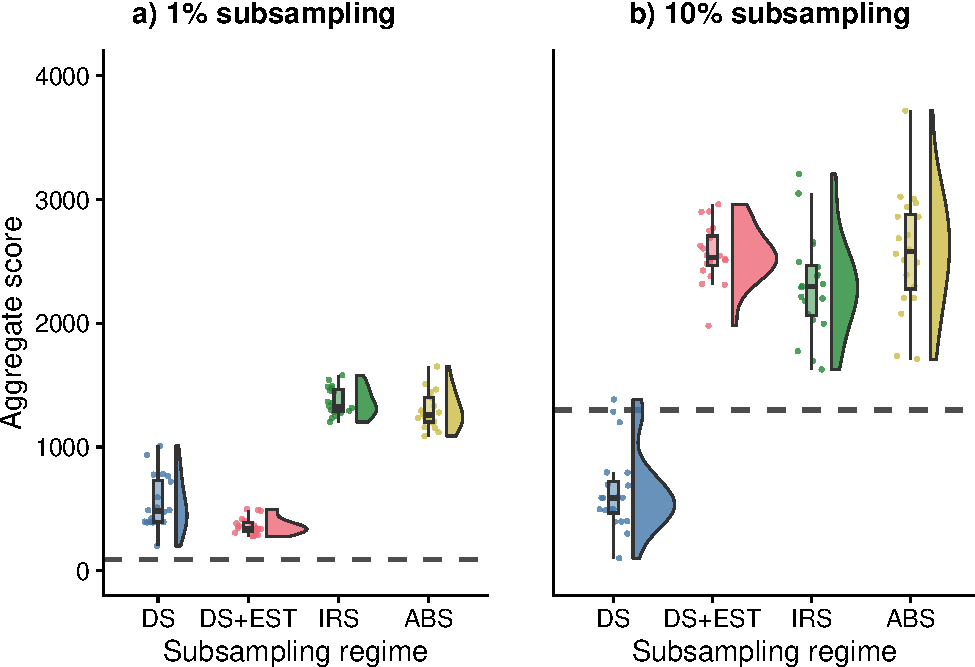
\includegraphics{phylogeny-informed-subsampling-supplemental_files/figure-latex/unnamed-chunk-64-1.pdf}

\begin{lstlisting}[language=R]
save_plot(
  filename = paste0(plot_directory, "2023-12-28-explore-lex-fig.pdf"),
  plot = lex_fig,
  base_width = 7,
  base_height = 3,
  dpi = 600
)
\end{lstlisting}

\hypertarget{program-synthesis-experiments}{%
\chapter{Program synthesis experiments}\label{program-synthesis-experiments}}

\begin{lstlisting}[language=R]
experiment_slug <- "2023-12-30-psynth"

working_directory <- paste0(
  "experiments/",
  experiment_slug,
  "/analysis/"
)

if (exists("bookdown_wd_prefix")) {
  working_directory <- paste0(
    bookdown_wd_prefix,
    working_directory
  )
}
\end{lstlisting}

\hypertarget{dependencies-3}{%
\section{Dependencies}\label{dependencies-3}}

\begin{lstlisting}[language=R]
library(tidyverse)
library(ggplot2)
library(cowplot)
library(RColorBrewer)
library(khroma)
library(rstatix)
library(knitr)
library(kableExtra)
\end{lstlisting}

\begin{lstlisting}
## 
## Attaching package: 'kableExtra'
\end{lstlisting}

\begin{lstlisting}
## The following object is masked from 'package:dplyr':
## 
##     group_rows
\end{lstlisting}

\begin{lstlisting}[language=R]
source("https://gist.githubusercontent.com/benmarwick/2a1bb0133ff568cbe28d/raw/fb53bd97121f7f9ce947837ef1a4c65a73bffb3f/geom_flat_violin.R")
\end{lstlisting}

\begin{lstlisting}[language=R]
print(version)
\end{lstlisting}

\begin{lstlisting}
##                _                           
## platform       aarch64-apple-darwin20      
## arch           aarch64                     
## os             darwin20                    
## system         aarch64, darwin20           
## status                                     
## major          4                           
## minor          2.1                         
## year           2022                        
## month          06                          
## day            23                          
## svn rev        82513                       
## language       R                           
## version.string R version 4.2.1 (2022-06-23)
## nickname       Funny-Looking Kid
\end{lstlisting}

\hypertarget{setup-3}{%
\section{Setup}\label{setup-3}}

\begin{lstlisting}[language=R]
# Configure our default graphing theme
theme_set(theme_cowplot())
# Create a directory to store plots
plot_directory <- paste0(working_directory, "plots/")
dir.create(plot_directory, showWarnings=FALSE)
\end{lstlisting}

\hypertarget{load-summary-data}{%
\subsection{Load summary data}\label{load-summary-data}}

\begin{lstlisting}[language=R]
summary_data_loc <- paste0(working_directory, "data/aggregate.csv")
summary_data <- read_csv(summary_data_loc)
\end{lstlisting}

\begin{lstlisting}
## Rows: 5000 Columns: 73
## -- Column specification -----------------------------------------------------------------------------------------------------------------------------------------------------------------------------------------
## Delimiter: ","
## chr (11): ANCESTOR_FILE_PATH, EVAL_FIT_EST_MODE, EVAL_MODE, POP_INIT_MODE, P...
## dbl (62): EVAL_CPU_CYCLES_PER_TEST, EVAL_MAX_PHYLO_SEARCH_DEPTH, MAX_ACTIVE_...
## 
## i Use `spec()` to retrieve the full column specification for this data.
## i Specify the column types or set `show_col_types = FALSE` to quiet this message.
\end{lstlisting}

\begin{lstlisting}[language=R]
summary_data <- summary_data %>%
  mutate(
    eval_mode_row = case_when(
      EVAL_MODE == "full" & TEST_DOWNSAMPLE_RATE == "1" ~ "down-sample",
      EVAL_MODE == "full" & NUM_COHORTS == "1" ~ "cohort",
      .default = EVAL_MODE
    ),
    evals_per_gen = case_when(
      EVAL_MODE == "cohort" ~ 1.0 / NUM_COHORTS,
      EVAL_MODE == "down-sample" ~ TEST_DOWNSAMPLE_RATE,
      EVAL_MODE == "indiv-rand-sample" ~ TEST_DOWNSAMPLE_RATE,
      EVAL_MODE == "phylo-informed-sample" ~ TEST_DOWNSAMPLE_RATE,
      EVAL_MODE == "full" ~ 1.0
    ),
    EVAL_FIT_EST_MODE = case_when(
      EVAL_FIT_EST_MODE == "ancestor-opt" ~ "ancestor",
      EVAL_FIT_EST_MODE == "relative-opt" ~ "relative",
      .default = EVAL_FIT_EST_MODE
    ),
    est_mode_with_depth = paste(
      EVAL_FIT_EST_MODE,
      EVAL_MAX_PHYLO_SEARCH_DEPTH,
      sep = "-"
    ),
    eval_mode_est_mode_depth = paste(
      EVAL_MODE,
      EVAL_FIT_EST_MODE,
      EVAL_MAX_PHYLO_SEARCH_DEPTH,
      sep = "-"
    ),
    .keep = "all"
  ) %>%
  mutate(
    eval_label = case_when(
      # Clean up down-sample label
      EVAL_MODE == "down-sample" & EVAL_FIT_EST_MODE != "none" ~ paste("down-sample", EVAL_FIT_EST_MODE, sep="-"),
      .default = EVAL_MODE
    ),
  ) %>%
  mutate(
    evals_per_gen = as.factor(evals_per_gen),
    est_mode_with_depth = as.factor(est_mode_with_depth),
    eval_mode_est_mode_depth = as.factor(eval_mode_est_mode_depth),
    EVAL_MAX_PHYLO_SEARCH_DEPTH = as.factor(EVAL_MAX_PHYLO_SEARCH_DEPTH),
    PROBLEM = as.factor(PROBLEM),
    SELECTION = as.factor(SELECTION),
    EVAL_MODE = as.factor(EVAL_MODE),
    NUM_COHORTS = as.factor(NUM_COHORTS),
    TEST_DOWNSAMPLE_RATE = as.factor(TEST_DOWNSAMPLE_RATE),
    EVAL_FIT_EST_MODE = factor(
      EVAL_FIT_EST_MODE,
      levels = c(
        "none",
        "ancestor",
        "relative"
      ),
      labels = c(
        "None",
        "Ancestor",
        "Relative"
      )
    ),
    .keep = "all"
  )

solution_counts <- summary_data %>%
  group_by(
    PROBLEM,
    evals_per_gen,
    eval_mode_row,
    EVAL_FIT_EST_MODE,
    est_mode_with_depth,
    eval_mode_est_mode_depth,
    EVAL_MODE,
    eval_label,
    EVAL_MAX_PHYLO_SEARCH_DEPTH
  ) %>%
  summarize(
    solution_count = sum(found_solution == "1"),
    replicates = n(),
    no_solution_count = n() - sum(found_solution == "1")
  )
\end{lstlisting}

\begin{lstlisting}
## `summarise()` has grouped output by 'PROBLEM', 'evals_per_gen', 'eval_mode_row', 'EVAL_FIT_EST_MODE', 'est_mode_with_depth', 'eval_mode_est_mode_depth', 'EVAL_MODE', 'eval_label'. You can override using the
## `.groups` argument.
\end{lstlisting}

\begin{lstlisting}[language=R]
# print(solution_counts, n=208)
solution_table <- kable(solution_counts) %>%
  kable_styling(latex_options = "striped", font_size = 25)
save_kable(solution_table, paste0(plot_directory, "solution_counts_table.pdf"))
solution_table
\end{lstlisting}

\begin{table}
\centering\begingroup\fontsize{25}{27}\selectfont

\begin{tabular}{l|l|l|l|l|l|l|l|l|r|r|r}
\hline
PROBLEM & evals\_per\_gen & eval\_mode\_row & EVAL\_FIT\_EST\_MODE & est\_mode\_with\_depth & eval\_mode\_est\_mode\_depth & EVAL\_MODE & eval\_label & EVAL\_MAX\_PHYLO\_SEARCH\_DEPTH & solution\_count & replicates & no\_solution\_count\\
\hline
\cellcolor{gray!6}{bouncing-balls} & \cellcolor{gray!6}{0.01} & \cellcolor{gray!6}{down-sample} & \cellcolor{gray!6}{None} & \cellcolor{gray!6}{none-1} & \cellcolor{gray!6}{down-sample-none-1} & \cellcolor{gray!6}{down-sample} & \cellcolor{gray!6}{down-sample} & \cellcolor{gray!6}{1} & \cellcolor{gray!6}{1} & \cellcolor{gray!6}{50} & \cellcolor{gray!6}{49}\\
\hline
bouncing-balls & 0.01 & down-sample & Ancestor & ancestor-8 & down-sample-ancestor-8 & down-sample & down-sample-ancestor & 8 & 8 & 50 & 42\\
\hline
\cellcolor{gray!6}{bouncing-balls} & \cellcolor{gray!6}{0.01} & \cellcolor{gray!6}{indiv-rand-sample} & \cellcolor{gray!6}{Ancestor} & \cellcolor{gray!6}{ancestor-8} & \cellcolor{gray!6}{indiv-rand-sample-ancestor-8} & \cellcolor{gray!6}{indiv-rand-sample} & \cellcolor{gray!6}{indiv-rand-sample} & \cellcolor{gray!6}{8} & \cellcolor{gray!6}{7} & \cellcolor{gray!6}{50} & \cellcolor{gray!6}{43}\\
\hline
bouncing-balls & 0.01 & phylo-informed-sample & Ancestor & ancestor-8 & phylo-informed-sample-ancestor-8 & phylo-informed-sample & phylo-informed-sample & 8 & 4 & 50 & 46\\
\hline
\cellcolor{gray!6}{bouncing-balls} & \cellcolor{gray!6}{0.1} & \cellcolor{gray!6}{down-sample} & \cellcolor{gray!6}{None} & \cellcolor{gray!6}{none-1} & \cellcolor{gray!6}{down-sample-none-1} & \cellcolor{gray!6}{down-sample} & \cellcolor{gray!6}{down-sample} & \cellcolor{gray!6}{1} & \cellcolor{gray!6}{0} & \cellcolor{gray!6}{50} & \cellcolor{gray!6}{50}\\
\hline
bouncing-balls & 0.1 & down-sample & Ancestor & ancestor-8 & down-sample-ancestor-8 & down-sample & down-sample-ancestor & 8 & 4 & 50 & 46\\
\hline
\cellcolor{gray!6}{bouncing-balls} & \cellcolor{gray!6}{0.1} & \cellcolor{gray!6}{indiv-rand-sample} & \cellcolor{gray!6}{Ancestor} & \cellcolor{gray!6}{ancestor-8} & \cellcolor{gray!6}{indiv-rand-sample-ancestor-8} & \cellcolor{gray!6}{indiv-rand-sample} & \cellcolor{gray!6}{indiv-rand-sample} & \cellcolor{gray!6}{8} & \cellcolor{gray!6}{2} & \cellcolor{gray!6}{50} & \cellcolor{gray!6}{48}\\
\hline
bouncing-balls & 0.1 & phylo-informed-sample & Ancestor & ancestor-8 & phylo-informed-sample-ancestor-8 & phylo-informed-sample & phylo-informed-sample & 8 & 3 & 50 & 47\\
\hline
\cellcolor{gray!6}{bouncing-balls} & \cellcolor{gray!6}{1} & \cellcolor{gray!6}{full} & \cellcolor{gray!6}{None} & \cellcolor{gray!6}{none-1} & \cellcolor{gray!6}{full-none-1} & \cellcolor{gray!6}{full} & \cellcolor{gray!6}{full} & \cellcolor{gray!6}{1} & \cellcolor{gray!6}{0} & \cellcolor{gray!6}{100} & \cellcolor{gray!6}{100}\\
\hline
dice-game & 0.01 & down-sample & None & none-1 & down-sample-none-1 & down-sample & down-sample & 1 & 0 & 50 & 50\\
\hline
\cellcolor{gray!6}{dice-game} & \cellcolor{gray!6}{0.01} & \cellcolor{gray!6}{down-sample} & \cellcolor{gray!6}{Ancestor} & \cellcolor{gray!6}{ancestor-8} & \cellcolor{gray!6}{down-sample-ancestor-8} & \cellcolor{gray!6}{down-sample} & \cellcolor{gray!6}{down-sample-ancestor} & \cellcolor{gray!6}{8} & \cellcolor{gray!6}{26} & \cellcolor{gray!6}{50} & \cellcolor{gray!6}{24}\\
\hline
dice-game & 0.01 & indiv-rand-sample & Ancestor & ancestor-8 & indiv-rand-sample-ancestor-8 & indiv-rand-sample & indiv-rand-sample & 8 & 25 & 50 & 25\\
\hline
\cellcolor{gray!6}{dice-game} & \cellcolor{gray!6}{0.01} & \cellcolor{gray!6}{phylo-informed-sample} & \cellcolor{gray!6}{Ancestor} & \cellcolor{gray!6}{ancestor-8} & \cellcolor{gray!6}{phylo-informed-sample-ancestor-8} & \cellcolor{gray!6}{phylo-informed-sample} & \cellcolor{gray!6}{phylo-informed-sample} & \cellcolor{gray!6}{8} & \cellcolor{gray!6}{31} & \cellcolor{gray!6}{50} & \cellcolor{gray!6}{19}\\
\hline
dice-game & 0.1 & down-sample & None & none-1 & down-sample-none-1 & down-sample & down-sample & 1 & 18 & 50 & 32\\
\hline
\cellcolor{gray!6}{dice-game} & \cellcolor{gray!6}{0.1} & \cellcolor{gray!6}{down-sample} & \cellcolor{gray!6}{Ancestor} & \cellcolor{gray!6}{ancestor-8} & \cellcolor{gray!6}{down-sample-ancestor-8} & \cellcolor{gray!6}{down-sample} & \cellcolor{gray!6}{down-sample-ancestor} & \cellcolor{gray!6}{8} & \cellcolor{gray!6}{19} & \cellcolor{gray!6}{50} & \cellcolor{gray!6}{31}\\
\hline
dice-game & 0.1 & indiv-rand-sample & Ancestor & ancestor-8 & indiv-rand-sample-ancestor-8 & indiv-rand-sample & indiv-rand-sample & 8 & 14 & 50 & 36\\
\hline
\cellcolor{gray!6}{dice-game} & \cellcolor{gray!6}{0.1} & \cellcolor{gray!6}{phylo-informed-sample} & \cellcolor{gray!6}{Ancestor} & \cellcolor{gray!6}{ancestor-8} & \cellcolor{gray!6}{phylo-informed-sample-ancestor-8} & \cellcolor{gray!6}{phylo-informed-sample} & \cellcolor{gray!6}{phylo-informed-sample} & \cellcolor{gray!6}{8} & \cellcolor{gray!6}{18} & \cellcolor{gray!6}{50} & \cellcolor{gray!6}{32}\\
\hline
dice-game & 1 & full & None & none-1 & full-none-1 & full & full & 1 & 0 & 100 & 100\\
\hline
\cellcolor{gray!6}{fizz-buzz} & \cellcolor{gray!6}{0.01} & \cellcolor{gray!6}{down-sample} & \cellcolor{gray!6}{None} & \cellcolor{gray!6}{none-1} & \cellcolor{gray!6}{down-sample-none-1} & \cellcolor{gray!6}{down-sample} & \cellcolor{gray!6}{down-sample} & \cellcolor{gray!6}{1} & \cellcolor{gray!6}{5} & \cellcolor{gray!6}{50} & \cellcolor{gray!6}{45}\\
\hline
fizz-buzz & 0.01 & down-sample & Ancestor & ancestor-8 & down-sample-ancestor-8 & down-sample & down-sample-ancestor & 8 & 10 & 50 & 40\\
\hline
\cellcolor{gray!6}{fizz-buzz} & \cellcolor{gray!6}{0.01} & \cellcolor{gray!6}{indiv-rand-sample} & \cellcolor{gray!6}{Ancestor} & \cellcolor{gray!6}{ancestor-8} & \cellcolor{gray!6}{indiv-rand-sample-ancestor-8} & \cellcolor{gray!6}{indiv-rand-sample} & \cellcolor{gray!6}{indiv-rand-sample} & \cellcolor{gray!6}{8} & \cellcolor{gray!6}{26} & \cellcolor{gray!6}{50} & \cellcolor{gray!6}{24}\\
\hline
fizz-buzz & 0.01 & phylo-informed-sample & Ancestor & ancestor-8 & phylo-informed-sample-ancestor-8 & phylo-informed-sample & phylo-informed-sample & 8 & 30 & 50 & 20\\
\hline
\cellcolor{gray!6}{fizz-buzz} & \cellcolor{gray!6}{0.1} & \cellcolor{gray!6}{down-sample} & \cellcolor{gray!6}{None} & \cellcolor{gray!6}{none-1} & \cellcolor{gray!6}{down-sample-none-1} & \cellcolor{gray!6}{down-sample} & \cellcolor{gray!6}{down-sample} & \cellcolor{gray!6}{1} & \cellcolor{gray!6}{39} & \cellcolor{gray!6}{50} & \cellcolor{gray!6}{11}\\
\hline
fizz-buzz & 0.1 & down-sample & Ancestor & ancestor-8 & down-sample-ancestor-8 & down-sample & down-sample-ancestor & 8 & 41 & 50 & 9\\
\hline
\cellcolor{gray!6}{fizz-buzz} & \cellcolor{gray!6}{0.1} & \cellcolor{gray!6}{indiv-rand-sample} & \cellcolor{gray!6}{Ancestor} & \cellcolor{gray!6}{ancestor-8} & \cellcolor{gray!6}{indiv-rand-sample-ancestor-8} & \cellcolor{gray!6}{indiv-rand-sample} & \cellcolor{gray!6}{indiv-rand-sample} & \cellcolor{gray!6}{8} & \cellcolor{gray!6}{19} & \cellcolor{gray!6}{50} & \cellcolor{gray!6}{31}\\
\hline
fizz-buzz & 0.1 & phylo-informed-sample & Ancestor & ancestor-8 & phylo-informed-sample-ancestor-8 & phylo-informed-sample & phylo-informed-sample & 8 & 24 & 50 & 26\\
\hline
\cellcolor{gray!6}{fizz-buzz} & \cellcolor{gray!6}{1} & \cellcolor{gray!6}{full} & \cellcolor{gray!6}{None} & \cellcolor{gray!6}{none-1} & \cellcolor{gray!6}{full-none-1} & \cellcolor{gray!6}{full} & \cellcolor{gray!6}{full} & \cellcolor{gray!6}{1} & \cellcolor{gray!6}{9} & \cellcolor{gray!6}{100} & \cellcolor{gray!6}{91}\\
\hline
for-loop-index & 0.01 & down-sample & None & none-1 & down-sample-none-1 & down-sample & down-sample & 1 & 6 & 50 & 44\\
\hline
\cellcolor{gray!6}{for-loop-index} & \cellcolor{gray!6}{0.01} & \cellcolor{gray!6}{down-sample} & \cellcolor{gray!6}{Ancestor} & \cellcolor{gray!6}{ancestor-8} & \cellcolor{gray!6}{down-sample-ancestor-8} & \cellcolor{gray!6}{down-sample} & \cellcolor{gray!6}{down-sample-ancestor} & \cellcolor{gray!6}{8} & \cellcolor{gray!6}{44} & \cellcolor{gray!6}{50} & \cellcolor{gray!6}{6}\\
\hline
for-loop-index & 0.01 & indiv-rand-sample & Ancestor & ancestor-8 & indiv-rand-sample-ancestor-8 & indiv-rand-sample & indiv-rand-sample & 8 & 49 & 50 & 1\\
\hline
\cellcolor{gray!6}{for-loop-index} & \cellcolor{gray!6}{0.01} & \cellcolor{gray!6}{phylo-informed-sample} & \cellcolor{gray!6}{Ancestor} & \cellcolor{gray!6}{ancestor-8} & \cellcolor{gray!6}{phylo-informed-sample-ancestor-8} & \cellcolor{gray!6}{phylo-informed-sample} & \cellcolor{gray!6}{phylo-informed-sample} & \cellcolor{gray!6}{8} & \cellcolor{gray!6}{50} & \cellcolor{gray!6}{50} & \cellcolor{gray!6}{0}\\
\hline
for-loop-index & 0.1 & down-sample & None & none-1 & down-sample-none-1 & down-sample & down-sample & 1 & 29 & 50 & 21\\
\hline
\cellcolor{gray!6}{for-loop-index} & \cellcolor{gray!6}{0.1} & \cellcolor{gray!6}{down-sample} & \cellcolor{gray!6}{Ancestor} & \cellcolor{gray!6}{ancestor-8} & \cellcolor{gray!6}{down-sample-ancestor-8} & \cellcolor{gray!6}{down-sample} & \cellcolor{gray!6}{down-sample-ancestor} & \cellcolor{gray!6}{8} & \cellcolor{gray!6}{35} & \cellcolor{gray!6}{50} & \cellcolor{gray!6}{15}\\
\hline
for-loop-index & 0.1 & indiv-rand-sample & Ancestor & ancestor-8 & indiv-rand-sample-ancestor-8 & indiv-rand-sample & indiv-rand-sample & 8 & 32 & 50 & 18\\
\hline
\cellcolor{gray!6}{for-loop-index} & \cellcolor{gray!6}{0.1} & \cellcolor{gray!6}{phylo-informed-sample} & \cellcolor{gray!6}{Ancestor} & \cellcolor{gray!6}{ancestor-8} & \cellcolor{gray!6}{phylo-informed-sample-ancestor-8} & \cellcolor{gray!6}{phylo-informed-sample} & \cellcolor{gray!6}{phylo-informed-sample} & \cellcolor{gray!6}{8} & \cellcolor{gray!6}{27} & \cellcolor{gray!6}{50} & \cellcolor{gray!6}{23}\\
\hline
for-loop-index & 1 & full & None & none-1 & full-none-1 & full & full & 1 & 24 & 100 & 76\\
\hline
\cellcolor{gray!6}{gcd} & \cellcolor{gray!6}{0.01} & \cellcolor{gray!6}{down-sample} & \cellcolor{gray!6}{None} & \cellcolor{gray!6}{none-1} & \cellcolor{gray!6}{down-sample-none-1} & \cellcolor{gray!6}{down-sample} & \cellcolor{gray!6}{down-sample} & \cellcolor{gray!6}{1} & \cellcolor{gray!6}{0} & \cellcolor{gray!6}{50} & \cellcolor{gray!6}{50}\\
\hline
gcd & 0.01 & down-sample & Ancestor & ancestor-8 & down-sample-ancestor-8 & down-sample & down-sample-ancestor & 8 & 12 & 50 & 38\\
\hline
\cellcolor{gray!6}{gcd} & \cellcolor{gray!6}{0.01} & \cellcolor{gray!6}{indiv-rand-sample} & \cellcolor{gray!6}{Ancestor} & \cellcolor{gray!6}{ancestor-8} & \cellcolor{gray!6}{indiv-rand-sample-ancestor-8} & \cellcolor{gray!6}{indiv-rand-sample} & \cellcolor{gray!6}{indiv-rand-sample} & \cellcolor{gray!6}{8} & \cellcolor{gray!6}{18} & \cellcolor{gray!6}{50} & \cellcolor{gray!6}{32}\\
\hline
gcd & 0.01 & phylo-informed-sample & Ancestor & ancestor-8 & phylo-informed-sample-ancestor-8 & phylo-informed-sample & phylo-informed-sample & 8 & 21 & 50 & 29\\
\hline
\cellcolor{gray!6}{gcd} & \cellcolor{gray!6}{0.1} & \cellcolor{gray!6}{down-sample} & \cellcolor{gray!6}{None} & \cellcolor{gray!6}{none-1} & \cellcolor{gray!6}{down-sample-none-1} & \cellcolor{gray!6}{down-sample} & \cellcolor{gray!6}{down-sample} & \cellcolor{gray!6}{1} & \cellcolor{gray!6}{2} & \cellcolor{gray!6}{50} & \cellcolor{gray!6}{48}\\
\hline
gcd & 0.1 & down-sample & Ancestor & ancestor-8 & down-sample-ancestor-8 & down-sample & down-sample-ancestor & 8 & 11 & 50 & 39\\
\hline
\cellcolor{gray!6}{gcd} & \cellcolor{gray!6}{0.1} & \cellcolor{gray!6}{indiv-rand-sample} & \cellcolor{gray!6}{Ancestor} & \cellcolor{gray!6}{ancestor-8} & \cellcolor{gray!6}{indiv-rand-sample-ancestor-8} & \cellcolor{gray!6}{indiv-rand-sample} & \cellcolor{gray!6}{indiv-rand-sample} & \cellcolor{gray!6}{8} & \cellcolor{gray!6}{12} & \cellcolor{gray!6}{50} & \cellcolor{gray!6}{38}\\
\hline
gcd & 0.1 & phylo-informed-sample & Ancestor & ancestor-8 & phylo-informed-sample-ancestor-8 & phylo-informed-sample & phylo-informed-sample & 8 & 12 & 50 & 38\\
\hline
\cellcolor{gray!6}{gcd} & \cellcolor{gray!6}{1} & \cellcolor{gray!6}{full} & \cellcolor{gray!6}{None} & \cellcolor{gray!6}{none-1} & \cellcolor{gray!6}{full-none-1} & \cellcolor{gray!6}{full} & \cellcolor{gray!6}{full} & \cellcolor{gray!6}{1} & \cellcolor{gray!6}{1} & \cellcolor{gray!6}{100} & \cellcolor{gray!6}{99}\\
\hline
grade & 0.01 & down-sample & None & none-1 & down-sample-none-1 & down-sample & down-sample & 1 & 2 & 50 & 48\\
\hline
\cellcolor{gray!6}{grade} & \cellcolor{gray!6}{0.01} & \cellcolor{gray!6}{down-sample} & \cellcolor{gray!6}{Ancestor} & \cellcolor{gray!6}{ancestor-8} & \cellcolor{gray!6}{down-sample-ancestor-8} & \cellcolor{gray!6}{down-sample} & \cellcolor{gray!6}{down-sample-ancestor} & \cellcolor{gray!6}{8} & \cellcolor{gray!6}{35} & \cellcolor{gray!6}{50} & \cellcolor{gray!6}{15}\\
\hline
grade & 0.01 & indiv-rand-sample & Ancestor & ancestor-8 & indiv-rand-sample-ancestor-8 & indiv-rand-sample & indiv-rand-sample & 8 & 40 & 50 & 10\\
\hline
\cellcolor{gray!6}{grade} & \cellcolor{gray!6}{0.01} & \cellcolor{gray!6}{phylo-informed-sample} & \cellcolor{gray!6}{Ancestor} & \cellcolor{gray!6}{ancestor-8} & \cellcolor{gray!6}{phylo-informed-sample-ancestor-8} & \cellcolor{gray!6}{phylo-informed-sample} & \cellcolor{gray!6}{phylo-informed-sample} & \cellcolor{gray!6}{8} & \cellcolor{gray!6}{41} & \cellcolor{gray!6}{50} & \cellcolor{gray!6}{9}\\
\hline
grade & 0.1 & down-sample & None & none-1 & down-sample-none-1 & down-sample & down-sample & 1 & 46 & 50 & 4\\
\hline
\cellcolor{gray!6}{grade} & \cellcolor{gray!6}{0.1} & \cellcolor{gray!6}{down-sample} & \cellcolor{gray!6}{Ancestor} & \cellcolor{gray!6}{ancestor-8} & \cellcolor{gray!6}{down-sample-ancestor-8} & \cellcolor{gray!6}{down-sample} & \cellcolor{gray!6}{down-sample-ancestor} & \cellcolor{gray!6}{8} & \cellcolor{gray!6}{40} & \cellcolor{gray!6}{50} & \cellcolor{gray!6}{10}\\
\hline
grade & 0.1 & indiv-rand-sample & Ancestor & ancestor-8 & indiv-rand-sample-ancestor-8 & indiv-rand-sample & indiv-rand-sample & 8 & 35 & 50 & 15\\
\hline
\cellcolor{gray!6}{grade} & \cellcolor{gray!6}{0.1} & \cellcolor{gray!6}{phylo-informed-sample} & \cellcolor{gray!6}{Ancestor} & \cellcolor{gray!6}{ancestor-8} & \cellcolor{gray!6}{phylo-informed-sample-ancestor-8} & \cellcolor{gray!6}{phylo-informed-sample} & \cellcolor{gray!6}{phylo-informed-sample} & \cellcolor{gray!6}{8} & \cellcolor{gray!6}{29} & \cellcolor{gray!6}{50} & \cellcolor{gray!6}{21}\\
\hline
grade & 1 & full & None & none-1 & full-none-1 & full & full & 1 & 22 & 100 & 78\\
\hline
\cellcolor{gray!6}{median} & \cellcolor{gray!6}{0.01} & \cellcolor{gray!6}{down-sample} & \cellcolor{gray!6}{None} & \cellcolor{gray!6}{none-1} & \cellcolor{gray!6}{down-sample-none-1} & \cellcolor{gray!6}{down-sample} & \cellcolor{gray!6}{down-sample} & \cellcolor{gray!6}{1} & \cellcolor{gray!6}{50} & \cellcolor{gray!6}{50} & \cellcolor{gray!6}{0}\\
\hline
median & 0.01 & down-sample & Ancestor & ancestor-8 & down-sample-ancestor-8 & down-sample & down-sample-ancestor & 8 & 40 & 50 & 10\\
\hline
\cellcolor{gray!6}{median} & \cellcolor{gray!6}{0.01} & \cellcolor{gray!6}{indiv-rand-sample} & \cellcolor{gray!6}{Ancestor} & \cellcolor{gray!6}{ancestor-8} & \cellcolor{gray!6}{indiv-rand-sample-ancestor-8} & \cellcolor{gray!6}{indiv-rand-sample} & \cellcolor{gray!6}{indiv-rand-sample} & \cellcolor{gray!6}{8} & \cellcolor{gray!6}{45} & \cellcolor{gray!6}{50} & \cellcolor{gray!6}{5}\\
\hline
median & 0.01 & phylo-informed-sample & Ancestor & ancestor-8 & phylo-informed-sample-ancestor-8 & phylo-informed-sample & phylo-informed-sample & 8 & 47 & 50 & 3\\
\hline
\cellcolor{gray!6}{median} & \cellcolor{gray!6}{0.1} & \cellcolor{gray!6}{down-sample} & \cellcolor{gray!6}{None} & \cellcolor{gray!6}{none-1} & \cellcolor{gray!6}{down-sample-none-1} & \cellcolor{gray!6}{down-sample} & \cellcolor{gray!6}{down-sample} & \cellcolor{gray!6}{1} & \cellcolor{gray!6}{47} & \cellcolor{gray!6}{50} & \cellcolor{gray!6}{3}\\
\hline
median & 0.1 & down-sample & Ancestor & ancestor-8 & down-sample-ancestor-8 & down-sample & down-sample-ancestor & 8 & 45 & 50 & 5\\
\hline
\cellcolor{gray!6}{median} & \cellcolor{gray!6}{0.1} & \cellcolor{gray!6}{indiv-rand-sample} & \cellcolor{gray!6}{Ancestor} & \cellcolor{gray!6}{ancestor-8} & \cellcolor{gray!6}{indiv-rand-sample-ancestor-8} & \cellcolor{gray!6}{indiv-rand-sample} & \cellcolor{gray!6}{indiv-rand-sample} & \cellcolor{gray!6}{8} & \cellcolor{gray!6}{47} & \cellcolor{gray!6}{50} & \cellcolor{gray!6}{3}\\
\hline
median & 0.1 & phylo-informed-sample & Ancestor & ancestor-8 & phylo-informed-sample-ancestor-8 & phylo-informed-sample & phylo-informed-sample & 8 & 40 & 50 & 10\\
\hline
\cellcolor{gray!6}{median} & \cellcolor{gray!6}{1} & \cellcolor{gray!6}{full} & \cellcolor{gray!6}{None} & \cellcolor{gray!6}{none-1} & \cellcolor{gray!6}{full-none-1} & \cellcolor{gray!6}{full} & \cellcolor{gray!6}{full} & \cellcolor{gray!6}{1} & \cellcolor{gray!6}{34} & \cellcolor{gray!6}{100} & \cellcolor{gray!6}{66}\\
\hline
small-or-large & 0.01 & down-sample & None & none-1 & down-sample-none-1 & down-sample & down-sample & 1 & 11 & 50 & 39\\
\hline
\cellcolor{gray!6}{small-or-large} & \cellcolor{gray!6}{0.01} & \cellcolor{gray!6}{down-sample} & \cellcolor{gray!6}{Ancestor} & \cellcolor{gray!6}{ancestor-8} & \cellcolor{gray!6}{down-sample-ancestor-8} & \cellcolor{gray!6}{down-sample} & \cellcolor{gray!6}{down-sample-ancestor} & \cellcolor{gray!6}{8} & \cellcolor{gray!6}{8} & \cellcolor{gray!6}{50} & \cellcolor{gray!6}{42}\\
\hline
small-or-large & 0.01 & indiv-rand-sample & Ancestor & ancestor-8 & indiv-rand-sample-ancestor-8 & indiv-rand-sample & indiv-rand-sample & 8 & 16 & 50 & 34\\
\hline
\cellcolor{gray!6}{small-or-large} & \cellcolor{gray!6}{0.01} & \cellcolor{gray!6}{phylo-informed-sample} & \cellcolor{gray!6}{Ancestor} & \cellcolor{gray!6}{ancestor-8} & \cellcolor{gray!6}{phylo-informed-sample-ancestor-8} & \cellcolor{gray!6}{phylo-informed-sample} & \cellcolor{gray!6}{phylo-informed-sample} & \cellcolor{gray!6}{8} & \cellcolor{gray!6}{14} & \cellcolor{gray!6}{50} & \cellcolor{gray!6}{36}\\
\hline
small-or-large & 0.1 & down-sample & None & none-1 & down-sample-none-1 & down-sample & down-sample & 1 & 28 & 50 & 22\\
\hline
\cellcolor{gray!6}{small-or-large} & \cellcolor{gray!6}{0.1} & \cellcolor{gray!6}{down-sample} & \cellcolor{gray!6}{Ancestor} & \cellcolor{gray!6}{ancestor-8} & \cellcolor{gray!6}{down-sample-ancestor-8} & \cellcolor{gray!6}{down-sample} & \cellcolor{gray!6}{down-sample-ancestor} & \cellcolor{gray!6}{8} & \cellcolor{gray!6}{21} & \cellcolor{gray!6}{50} & \cellcolor{gray!6}{29}\\
\hline
small-or-large & 0.1 & indiv-rand-sample & Ancestor & ancestor-8 & indiv-rand-sample-ancestor-8 & indiv-rand-sample & indiv-rand-sample & 8 & 8 & 50 & 42\\
\hline
\cellcolor{gray!6}{small-or-large} & \cellcolor{gray!6}{0.1} & \cellcolor{gray!6}{phylo-informed-sample} & \cellcolor{gray!6}{Ancestor} & \cellcolor{gray!6}{ancestor-8} & \cellcolor{gray!6}{phylo-informed-sample-ancestor-8} & \cellcolor{gray!6}{phylo-informed-sample} & \cellcolor{gray!6}{phylo-informed-sample} & \cellcolor{gray!6}{8} & \cellcolor{gray!6}{12} & \cellcolor{gray!6}{50} & \cellcolor{gray!6}{38}\\
\hline
small-or-large & 1 & full & None & none-1 & full-none-1 & full & full & 1 & 4 & 100 & 96\\
\hline
\cellcolor{gray!6}{smallest} & \cellcolor{gray!6}{0.01} & \cellcolor{gray!6}{down-sample} & \cellcolor{gray!6}{None} & \cellcolor{gray!6}{none-1} & \cellcolor{gray!6}{down-sample-none-1} & \cellcolor{gray!6}{down-sample} & \cellcolor{gray!6}{down-sample} & \cellcolor{gray!6}{1} & \cellcolor{gray!6}{49} & \cellcolor{gray!6}{50} & \cellcolor{gray!6}{1}\\
\hline
smallest & 0.01 & down-sample & Ancestor & ancestor-8 & down-sample-ancestor-8 & down-sample & down-sample-ancestor & 8 & 47 & 50 & 3\\
\hline
\cellcolor{gray!6}{smallest} & \cellcolor{gray!6}{0.01} & \cellcolor{gray!6}{indiv-rand-sample} & \cellcolor{gray!6}{Ancestor} & \cellcolor{gray!6}{ancestor-8} & \cellcolor{gray!6}{indiv-rand-sample-ancestor-8} & \cellcolor{gray!6}{indiv-rand-sample} & \cellcolor{gray!6}{indiv-rand-sample} & \cellcolor{gray!6}{8} & \cellcolor{gray!6}{50} & \cellcolor{gray!6}{50} & \cellcolor{gray!6}{0}\\
\hline
smallest & 0.01 & phylo-informed-sample & Ancestor & ancestor-8 & phylo-informed-sample-ancestor-8 & phylo-informed-sample & phylo-informed-sample & 8 & 50 & 50 & 0\\
\hline
\cellcolor{gray!6}{smallest} & \cellcolor{gray!6}{0.1} & \cellcolor{gray!6}{down-sample} & \cellcolor{gray!6}{None} & \cellcolor{gray!6}{none-1} & \cellcolor{gray!6}{down-sample-none-1} & \cellcolor{gray!6}{down-sample} & \cellcolor{gray!6}{down-sample} & \cellcolor{gray!6}{1} & \cellcolor{gray!6}{47} & \cellcolor{gray!6}{50} & \cellcolor{gray!6}{3}\\
\hline
smallest & 0.1 & down-sample & Ancestor & ancestor-8 & down-sample-ancestor-8 & down-sample & down-sample-ancestor & 8 & 47 & 50 & 3\\
\hline
\cellcolor{gray!6}{smallest} & \cellcolor{gray!6}{0.1} & \cellcolor{gray!6}{indiv-rand-sample} & \cellcolor{gray!6}{Ancestor} & \cellcolor{gray!6}{ancestor-8} & \cellcolor{gray!6}{indiv-rand-sample-ancestor-8} & \cellcolor{gray!6}{indiv-rand-sample} & \cellcolor{gray!6}{indiv-rand-sample} & \cellcolor{gray!6}{8} & \cellcolor{gray!6}{49} & \cellcolor{gray!6}{50} & \cellcolor{gray!6}{1}\\
\hline
smallest & 0.1 & phylo-informed-sample & Ancestor & ancestor-8 & phylo-informed-sample-ancestor-8 & phylo-informed-sample & phylo-informed-sample & 8 & 49 & 50 & 1\\
\hline
\cellcolor{gray!6}{smallest} & \cellcolor{gray!6}{1} & \cellcolor{gray!6}{full} & \cellcolor{gray!6}{None} & \cellcolor{gray!6}{none-1} & \cellcolor{gray!6}{full-none-1} & \cellcolor{gray!6}{full} & \cellcolor{gray!6}{full} & \cellcolor{gray!6}{1} & \cellcolor{gray!6}{51} & \cellcolor{gray!6}{100} & \cellcolor{gray!6}{49}\\
\hline
snow-day & 0.01 & down-sample & None & none-1 & down-sample-none-1 & down-sample & down-sample & 1 & 0 & 50 & 50\\
\hline
\cellcolor{gray!6}{snow-day} & \cellcolor{gray!6}{0.01} & \cellcolor{gray!6}{down-sample} & \cellcolor{gray!6}{Ancestor} & \cellcolor{gray!6}{ancestor-8} & \cellcolor{gray!6}{down-sample-ancestor-8} & \cellcolor{gray!6}{down-sample} & \cellcolor{gray!6}{down-sample-ancestor} & \cellcolor{gray!6}{8} & \cellcolor{gray!6}{3} & \cellcolor{gray!6}{50} & \cellcolor{gray!6}{47}\\
\hline
snow-day & 0.01 & indiv-rand-sample & Ancestor & ancestor-8 & indiv-rand-sample-ancestor-8 & indiv-rand-sample & indiv-rand-sample & 8 & 1 & 50 & 49\\
\hline
\cellcolor{gray!6}{snow-day} & \cellcolor{gray!6}{0.01} & \cellcolor{gray!6}{phylo-informed-sample} & \cellcolor{gray!6}{Ancestor} & \cellcolor{gray!6}{ancestor-8} & \cellcolor{gray!6}{phylo-informed-sample-ancestor-8} & \cellcolor{gray!6}{phylo-informed-sample} & \cellcolor{gray!6}{phylo-informed-sample} & \cellcolor{gray!6}{8} & \cellcolor{gray!6}{1} & \cellcolor{gray!6}{50} & \cellcolor{gray!6}{49}\\
\hline
snow-day & 0.1 & down-sample & None & none-1 & down-sample-none-1 & down-sample & down-sample & 1 & 0 & 50 & 50\\
\hline
\cellcolor{gray!6}{snow-day} & \cellcolor{gray!6}{0.1} & \cellcolor{gray!6}{down-sample} & \cellcolor{gray!6}{Ancestor} & \cellcolor{gray!6}{ancestor-8} & \cellcolor{gray!6}{down-sample-ancestor-8} & \cellcolor{gray!6}{down-sample} & \cellcolor{gray!6}{down-sample-ancestor} & \cellcolor{gray!6}{8} & \cellcolor{gray!6}{0} & \cellcolor{gray!6}{50} & \cellcolor{gray!6}{50}\\
\hline
snow-day & 0.1 & indiv-rand-sample & Ancestor & ancestor-8 & indiv-rand-sample-ancestor-8 & indiv-rand-sample & indiv-rand-sample & 8 & 1 & 50 & 49\\
\hline
\cellcolor{gray!6}{snow-day} & \cellcolor{gray!6}{0.1} & \cellcolor{gray!6}{phylo-informed-sample} & \cellcolor{gray!6}{Ancestor} & \cellcolor{gray!6}{ancestor-8} & \cellcolor{gray!6}{phylo-informed-sample-ancestor-8} & \cellcolor{gray!6}{phylo-informed-sample} & \cellcolor{gray!6}{phylo-informed-sample} & \cellcolor{gray!6}{8} & \cellcolor{gray!6}{4} & \cellcolor{gray!6}{50} & \cellcolor{gray!6}{46}\\
\hline
snow-day & 1 & full & None & none-1 & full-none-1 & full & full & 1 & 0 & 100 & 100\\
\hline
\end{tabular}
\endgroup{}
\end{table}

\begin{lstlisting}[language=R]
# Summarize avg num selected
# -- Not totally great because weird stuff happens when a solution is found (population collapses, etc)
ts_data_loc <- paste0(working_directory, "data/time_series.csv")
ts_data <- read_csv(ts_data_loc)
\end{lstlisting}

\begin{lstlisting}
## Rows: 99773 Columns: 24
## -- Column specification -----------------------------------------------------------------------------------------------------------------------------------------------------------------------------------------
## Delimiter: ","
## chr  (6): EVAL_FIT_EST_MODE, EVAL_MODE, PROBLEM, SELECTION, TESTING_SET_PATH...
## dbl (18): EVAL_MAX_PHYLO_SEARCH_DEPTH, NUM_COHORTS, SEED, TEST_DOWNSAMPLE_RA...
## 
## i Use `spec()` to retrieve the full column specification for this data.
## i Specify the column types or set `show_col_types = FALSE` to quiet this message.
\end{lstlisting}

\begin{lstlisting}[language=R]
ts_data <- ts_data %>%
  mutate(
    eval_mode_row = case_when(
      EVAL_MODE == "full" & TEST_DOWNSAMPLE_RATE == "1" ~ "down-sample",
      EVAL_MODE == "full" & NUM_COHORTS == "1" ~ "cohort",
      .default = EVAL_MODE
    ),
    evals_per_gen = case_when(
      EVAL_MODE == "cohort" ~ 1.0 / NUM_COHORTS,
      EVAL_MODE == "down-sample" ~ TEST_DOWNSAMPLE_RATE,
      EVAL_MODE == "indiv-rand-sample" ~ TEST_DOWNSAMPLE_RATE,
      EVAL_MODE == "phylo-informed-sample" ~ TEST_DOWNSAMPLE_RATE,
      EVAL_MODE == "full" ~ 1.0
    ),
    EVAL_FIT_EST_MODE = case_when(
      EVAL_FIT_EST_MODE == "ancestor-opt" ~ "ancestor",
      EVAL_FIT_EST_MODE == "relative-opt" ~ "relative",
      .default = EVAL_FIT_EST_MODE
    ),
    est_mode_with_depth = paste(
      EVAL_FIT_EST_MODE,
      EVAL_MAX_PHYLO_SEARCH_DEPTH,
      sep = "-"
    ),
    eval_mode_est_mode_depth = paste(
      EVAL_MODE,
      EVAL_FIT_EST_MODE,
      EVAL_MAX_PHYLO_SEARCH_DEPTH,
      sep = "-"
    ),
    .keep = "all"
  ) %>%
  mutate(
    eval_label = case_when(
      # Clean up down-sample label
      EVAL_MODE == "down-sample" & EVAL_FIT_EST_MODE != "none" ~ paste("down-sample", EVAL_FIT_EST_MODE, sep="-"),
      .default = EVAL_MODE
    ),
  ) %>%
  mutate(
    evals_per_gen = as.factor(evals_per_gen),
    est_mode_with_depth = as.factor(est_mode_with_depth),
    eval_mode_est_mode_depth = as.factor(eval_mode_est_mode_depth),
    EVAL_MAX_PHYLO_SEARCH_DEPTH = as.factor(EVAL_MAX_PHYLO_SEARCH_DEPTH),
    PROBLEM = as.factor(PROBLEM),
    SELECTION = as.factor(SELECTION),
    EVAL_MODE = as.factor(EVAL_MODE),
    NUM_COHORTS = as.factor(NUM_COHORTS),
    TEST_DOWNSAMPLE_RATE = as.factor(TEST_DOWNSAMPLE_RATE),
    EVAL_FIT_EST_MODE = factor(
      EVAL_FIT_EST_MODE,
      levels = c(
        "none",
        "ancestor",
        "relative"
      ),
      labels = c(
        "None",
        "Ancestor",
        "Relative"
      )
    ),
    .keep = "all"
  )

ts_avgs <- ts_data %>%
  group_by(
    SEED,
    eval_label,
    evals_per_gen,
    PROBLEM
  ) %>%
  summarize(
    n = n(),
    avg_num_unique_selected = mean(num_unique_selected),
    avg_entropy_selected_ids = mean(entropy_selected_ids)
  ) %>%
  mutate(
    eval_label = as.factor(eval_label),
    evals_per_gen = as.factor(evals_per_gen),
    PROBLEM = as.factor(PROBLEM)
  )
\end{lstlisting}

\begin{lstlisting}
## `summarise()` has grouped output by 'SEED', 'eval_label', 'evals_per_gen'. You
## can override using the `.groups` argument.
\end{lstlisting}

\hypertarget{problem-solving-success-statistics}{%
\section{Problem-solving success statistics}\label{problem-solving-success-statistics}}

\begin{lstlisting}[language=R]
sol_stats_data <- solution_counts %>%
  filter(EVAL_MODE != "full") %>%
  ungroup() %>%
  unite(
    "grouping",
    PROBLEM,
    evals_per_gen,
    sep="_"
  ) %>%
  select(
    grouping, eval_label, solution_count, no_solution_count
  ) %>%
  mutate(
    grouping = as.factor(grouping)
  )
\end{lstlisting}

\begin{lstlisting}[language=R]
fisher_results <- data.frame(
  comparison = character(),
  group1 = character(),
  group2 = character(),
  n = integer(),
  p = double(),
  p.adj = double(),
  p.adj.signif = character()
)

groupings <- levels(sol_stats_data$grouping)
for (g in groupings) {

  ft_results <- sol_stats_data %>%
    filter(grouping == g) %>%
    select(!grouping) %>%
    column_to_rownames(var = "eval_label") %>%
    pairwise_fisher_test(
      p.adjust.method = "holm"
    ) %>%
    add_significance("p.adj")

  ft_results <- ft_results %>%
    mutate(
      comparison = rep(g, nrow(ft_results)),
      .keep = "all"
    ) %>%
    relocate(comparison)

  fisher_results <- rbind(
    fisher_results,
    ft_results
  )
}
fisher_results <- as.tibble(fisher_results)
\end{lstlisting}

\begin{lstlisting}
## Warning: `as.tibble()` was deprecated in tibble 2.0.0.
## i Please use `as_tibble()` instead.
## i The signature and semantics have changed, see `?as_tibble`.
## This warning is displayed once every 8 hours.
## Call `lifecycle::last_lifecycle_warnings()` to see where this warning was generated.
\end{lstlisting}

\begin{lstlisting}[language=R]
fisher_results <- fisher_results %>%
  mutate(
    comparison = as.factor(comparison),
    group1 = as.factor(group1),
    group2 = as.factor(group2),
  ) %>%
  group_by(
    comparison
  )

fisher_table <- kbl(fisher_results) %>% kable_styling()
save_kable(fisher_table, paste0(plot_directory, "stats_table.pdf"))
fisher_table
\end{lstlisting}

\begin{table}
\centering
\begin{tabular}[t]{l|l|l|r|r|r|l}
\hline
comparison & group1 & group2 & n & p & p.adj & p.adj.signif\\
\hline
bouncing-balls\_0.01 & down-sample & down-sample-ancestor & 100 & 3.09e-02 & 1.85e-01 & ns\\
\hline
bouncing-balls\_0.01 & down-sample & indiv-rand-sample & 100 & 5.94e-02 & 2.97e-01 & ns\\
\hline
bouncing-balls\_0.01 & down-sample & phylo-informed-sample & 100 & 3.62e-01 & 1.00e+00 & ns\\
\hline
bouncing-balls\_0.01 & down-sample-ancestor & indiv-rand-sample & 100 & 1.00e+00 & 1.00e+00 & ns\\
\hline
bouncing-balls\_0.01 & down-sample-ancestor & phylo-informed-sample & 100 & 3.57e-01 & 1.00e+00 & ns\\
\hline
bouncing-balls\_0.01 & indiv-rand-sample & phylo-informed-sample & 100 & 5.25e-01 & 1.00e+00 & ns\\
\hline
bouncing-balls\_0.1 & down-sample & down-sample-ancestor & 100 & 1.17e-01 & 7.02e-01 & ns\\
\hline
bouncing-balls\_0.1 & down-sample & indiv-rand-sample & 100 & 4.95e-01 & 1.00e+00 & ns\\
\hline
bouncing-balls\_0.1 & down-sample & phylo-informed-sample & 100 & 2.42e-01 & 1.00e+00 & ns\\
\hline
bouncing-balls\_0.1 & down-sample-ancestor & indiv-rand-sample & 100 & 6.78e-01 & 1.00e+00 & ns\\
\hline
bouncing-balls\_0.1 & down-sample-ancestor & phylo-informed-sample & 100 & 1.00e+00 & 1.00e+00 & ns\\
\hline
bouncing-balls\_0.1 & indiv-rand-sample & phylo-informed-sample & 100 & 1.00e+00 & 1.00e+00 & ns\\
\hline
dice-game\_0.01 & down-sample & down-sample-ancestor & 100 & 0.00e+00 & 0.00e+00 & ****\\
\hline
dice-game\_0.01 & down-sample & indiv-rand-sample & 100 & 0.00e+00 & 0.00e+00 & ****\\
\hline
dice-game\_0.01 & down-sample & phylo-informed-sample & 100 & 0.00e+00 & 0.00e+00 & ****\\
\hline
dice-game\_0.01 & down-sample-ancestor & indiv-rand-sample & 100 & 1.00e+00 & 1.00e+00 & ns\\
\hline
dice-game\_0.01 & down-sample-ancestor & phylo-informed-sample & 100 & 4.19e-01 & 9.42e-01 & ns\\
\hline
dice-game\_0.01 & indiv-rand-sample & phylo-informed-sample & 100 & 3.14e-01 & 9.42e-01 & ns\\
\hline
dice-game\_0.1 & down-sample & down-sample-ancestor & 100 & 1.00e+00 & 1.00e+00 & ns\\
\hline
dice-game\_0.1 & down-sample & indiv-rand-sample & 100 & 5.21e-01 & 1.00e+00 & ns\\
\hline
dice-game\_0.1 & down-sample & phylo-informed-sample & 100 & 1.00e+00 & 1.00e+00 & ns\\
\hline
dice-game\_0.1 & down-sample-ancestor & indiv-rand-sample & 100 & 3.95e-01 & 1.00e+00 & ns\\
\hline
dice-game\_0.1 & down-sample-ancestor & phylo-informed-sample & 100 & 1.00e+00 & 1.00e+00 & ns\\
\hline
dice-game\_0.1 & indiv-rand-sample & phylo-informed-sample & 100 & 5.21e-01 & 1.00e+00 & ns\\
\hline
fizz-buzz\_0.01 & down-sample & down-sample-ancestor & 100 & 2.62e-01 & 5.24e-01 & ns\\
\hline
fizz-buzz\_0.01 & down-sample & indiv-rand-sample & 100 & 8.60e-06 & 4.28e-05 & ****\\
\hline
fizz-buzz\_0.01 & down-sample & phylo-informed-sample & 100 & 2.00e-07 & 1.20e-06 & ****\\
\hline
fizz-buzz\_0.01 & down-sample-ancestor & indiv-rand-sample & 100 & 1.59e-03 & 4.77e-03 & **\\
\hline
fizz-buzz\_0.01 & down-sample-ancestor & phylo-informed-sample & 100 & 8.31e-05 & 3.32e-04 & ***\\
\hline
fizz-buzz\_0.01 & indiv-rand-sample & phylo-informed-sample & 100 & 5.46e-01 & 5.46e-01 & ns\\
\hline
fizz-buzz\_0.1 & down-sample & down-sample-ancestor & 100 & 8.03e-01 & 8.38e-01 & ns\\
\hline
fizz-buzz\_0.1 & down-sample & indiv-rand-sample & 100 & 9.55e-05 & 4.78e-04 & ***\\
\hline
fizz-buzz\_0.1 & down-sample & phylo-informed-sample & 100 & 3.46e-03 & 1.04e-02 & *\\
\hline
fizz-buzz\_0.1 & down-sample-ancestor & indiv-rand-sample & 100 & 1.26e-05 & 7.56e-05 & ****\\
\hline
fizz-buzz\_0.1 & down-sample-ancestor & phylo-informed-sample & 100 & 6.80e-04 & 2.72e-03 & **\\
\hline
fizz-buzz\_0.1 & indiv-rand-sample & phylo-informed-sample & 100 & 4.19e-01 & 8.38e-01 & ns\\
\hline
for-loop-index\_0.01 & down-sample & down-sample-ancestor & 100 & 0.00e+00 & 0.00e+00 & ****\\
\hline
for-loop-index\_0.01 & down-sample & indiv-rand-sample & 100 & 0.00e+00 & 0.00e+00 & ****\\
\hline
for-loop-index\_0.01 & down-sample & phylo-informed-sample & 100 & 0.00e+00 & 0.00e+00 & ****\\
\hline
for-loop-index\_0.01 & down-sample-ancestor & indiv-rand-sample & 100 & 1.12e-01 & 2.24e-01 & ns\\
\hline
for-loop-index\_0.01 & down-sample-ancestor & phylo-informed-sample & 100 & 2.67e-02 & 8.01e-02 & ns\\
\hline
for-loop-index\_0.01 & indiv-rand-sample & phylo-informed-sample & 100 & 1.00e+00 & 1.00e+00 & ns\\
\hline
for-loop-index\_0.1 & down-sample & down-sample-ancestor & 100 & 2.98e-01 & 1.00e+00 & ns\\
\hline
for-loop-index\_0.1 & down-sample & indiv-rand-sample & 100 & 6.82e-01 & 1.00e+00 & ns\\
\hline
for-loop-index\_0.1 & down-sample & phylo-informed-sample & 100 & 8.40e-01 & 1.00e+00 & ns\\
\hline
for-loop-index\_0.1 & down-sample-ancestor & indiv-rand-sample & 100 & 6.71e-01 & 1.00e+00 & ns\\
\hline
for-loop-index\_0.1 & down-sample-ancestor & phylo-informed-sample & 100 & 1.49e-01 & 8.94e-01 & ns\\
\hline
for-loop-index\_0.1 & indiv-rand-sample & phylo-informed-sample & 100 & 4.16e-01 & 1.00e+00 & ns\\
\hline
gcd\_0.01 & down-sample & down-sample-ancestor & 100 & 2.31e-04 & 9.24e-04 & ***\\
\hline
gcd\_0.01 & down-sample & indiv-rand-sample & 100 & 1.20e-06 & 5.90e-06 & ****\\
\hline
gcd\_0.01 & down-sample & phylo-informed-sample & 100 & 1.00e-07 & 4.00e-07 & ****\\
\hline
gcd\_0.01 & down-sample-ancestor & indiv-rand-sample & 100 & 2.75e-01 & 5.50e-01 & ns\\
\hline
gcd\_0.01 & down-sample-ancestor & phylo-informed-sample & 100 & 8.81e-02 & 2.64e-01 & ns\\
\hline
gcd\_0.01 & indiv-rand-sample & phylo-informed-sample & 100 & 6.82e-01 & 6.82e-01 & ns\\
\hline
gcd\_0.1 & down-sample & down-sample-ancestor & 100 & 1.47e-02 & 5.88e-02 & ns\\
\hline
gcd\_0.1 & down-sample & indiv-rand-sample & 100 & 7.58e-03 & 4.55e-02 & *\\
\hline
gcd\_0.1 & down-sample & phylo-informed-sample & 100 & 7.58e-03 & 4.55e-02 & *\\
\hline
gcd\_0.1 & down-sample-ancestor & indiv-rand-sample & 100 & 1.00e+00 & 1.00e+00 & ns\\
\hline
gcd\_0.1 & down-sample-ancestor & phylo-informed-sample & 100 & 1.00e+00 & 1.00e+00 & ns\\
\hline
gcd\_0.1 & indiv-rand-sample & phylo-informed-sample & 100 & 1.00e+00 & 1.00e+00 & ns\\
\hline
grade\_0.01 & down-sample & down-sample-ancestor & 100 & 0.00e+00 & 0.00e+00 & ****\\
\hline
grade\_0.01 & down-sample & indiv-rand-sample & 100 & 0.00e+00 & 0.00e+00 & ****\\
\hline
grade\_0.01 & down-sample & phylo-informed-sample & 100 & 0.00e+00 & 0.00e+00 & ****\\
\hline
grade\_0.01 & down-sample-ancestor & indiv-rand-sample & 100 & 3.56e-01 & 7.23e-01 & ns\\
\hline
grade\_0.01 & down-sample-ancestor & phylo-informed-sample & 100 & 2.41e-01 & 7.23e-01 & ns\\
\hline
grade\_0.01 & indiv-rand-sample & phylo-informed-sample & 100 & 1.00e+00 & 1.00e+00 & ns\\
\hline
grade\_0.1 & down-sample & down-sample-ancestor & 100 & 1.48e-01 & 4.44e-01 & ns\\
\hline
grade\_0.1 & down-sample & indiv-rand-sample & 100 & 9.49e-03 & 4.74e-02 & *\\
\hline
grade\_0.1 & down-sample & phylo-informed-sample & 100 & 1.43e-04 & 8.58e-04 & ***\\
\hline
grade\_0.1 & down-sample-ancestor & indiv-rand-sample & 100 & 3.56e-01 & 5.96e-01 & ns\\
\hline
grade\_0.1 & down-sample-ancestor & phylo-informed-sample & 100 & 2.97e-02 & 1.19e-01 & ns\\
\hline
grade\_0.1 & indiv-rand-sample & phylo-informed-sample & 100 & 2.98e-01 & 5.96e-01 & ns\\
\hline
median\_0.01 & down-sample & down-sample-ancestor & 100 & 1.19e-03 & 7.14e-03 & **\\
\hline
median\_0.01 & down-sample & indiv-rand-sample & 100 & 5.63e-02 & 2.82e-01 & ns\\
\hline
median\_0.01 & down-sample & phylo-informed-sample & 100 & 2.42e-01 & 7.26e-01 & ns\\
\hline
median\_0.01 & down-sample-ancestor & indiv-rand-sample & 100 & 2.62e-01 & 7.26e-01 & ns\\
\hline
median\_0.01 & down-sample-ancestor & phylo-informed-sample & 100 & 7.13e-02 & 2.85e-01 & ns\\
\hline
median\_0.01 & indiv-rand-sample & phylo-informed-sample & 100 & 7.15e-01 & 7.26e-01 & ns\\
\hline
median\_0.1 & down-sample & down-sample-ancestor & 100 & 7.15e-01 & 1.00e+00 & ns\\
\hline
median\_0.1 & down-sample & indiv-rand-sample & 100 & 1.00e+00 & 1.00e+00 & ns\\
\hline
median\_0.1 & down-sample & phylo-informed-sample & 100 & 7.13e-02 & 4.28e-01 & ns\\
\hline
median\_0.1 & down-sample-ancestor & indiv-rand-sample & 100 & 7.15e-01 & 1.00e+00 & ns\\
\hline
median\_0.1 & down-sample-ancestor & phylo-informed-sample & 100 & 2.62e-01 & 1.00e+00 & ns\\
\hline
median\_0.1 & indiv-rand-sample & phylo-informed-sample & 100 & 7.13e-02 & 4.28e-01 & ns\\
\hline
small-or-large\_0.01 & down-sample & down-sample-ancestor & 100 & 6.11e-01 & 1.00e+00 & ns\\
\hline
small-or-large\_0.01 & down-sample & indiv-rand-sample & 100 & 3.68e-01 & 1.00e+00 & ns\\
\hline
small-or-large\_0.01 & down-sample & phylo-informed-sample & 100 & 6.45e-01 & 1.00e+00 & ns\\
\hline
small-or-large\_0.01 & down-sample-ancestor & indiv-rand-sample & 100 & 1.00e-01 & 6.00e-01 & ns\\
\hline
small-or-large\_0.01 & down-sample-ancestor & phylo-informed-sample & 100 & 2.27e-01 & 1.00e+00 & ns\\
\hline
small-or-large\_0.01 & indiv-rand-sample & phylo-informed-sample & 100 & 8.28e-01 & 1.00e+00 & ns\\
\hline
small-or-large\_0.1 & down-sample & down-sample-ancestor & 100 & 2.30e-01 & 4.60e-01 & ns\\
\hline
small-or-large\_0.1 & down-sample & indiv-rand-sample & 100 & 5.58e-05 & 3.35e-04 & ***\\
\hline
small-or-large\_0.1 & down-sample & phylo-informed-sample & 100 & 2.02e-03 & 1.01e-02 & *\\
\hline
small-or-large\_0.1 & down-sample-ancestor & indiv-rand-sample & 100 & 7.58e-03 & 3.03e-02 & *\\
\hline
small-or-large\_0.1 & down-sample-ancestor & phylo-informed-sample & 100 & 8.81e-02 & 2.64e-01 & ns\\
\hline
small-or-large\_0.1 & indiv-rand-sample & phylo-informed-sample & 100 & 4.54e-01 & 4.60e-01 & ns\\
\hline
smallest\_0.01 & down-sample & down-sample-ancestor & 100 & 6.17e-01 & 1.00e+00 & ns\\
\hline
smallest\_0.01 & down-sample & indiv-rand-sample & 100 & 1.00e+00 & 1.00e+00 & ns\\
\hline
smallest\_0.01 & down-sample & phylo-informed-sample & 100 & 1.00e+00 & 1.00e+00 & ns\\
\hline
smallest\_0.01 & down-sample-ancestor & indiv-rand-sample & 100 & 2.42e-01 & 1.00e+00 & ns\\
\hline
smallest\_0.01 & down-sample-ancestor & phylo-informed-sample & 100 & 2.42e-01 & 1.00e+00 & ns\\
\hline
smallest\_0.01 & indiv-rand-sample & phylo-informed-sample & 100 & 1.00e+00 & 1.00e+00 & ns\\
\hline
smallest\_0.1 & down-sample & down-sample-ancestor & 100 & 1.00e+00 & 1.00e+00 & ns\\
\hline
smallest\_0.1 & down-sample & indiv-rand-sample & 100 & 6.17e-01 & 1.00e+00 & ns\\
\hline
smallest\_0.1 & down-sample & phylo-informed-sample & 100 & 6.17e-01 & 1.00e+00 & ns\\
\hline
smallest\_0.1 & down-sample-ancestor & indiv-rand-sample & 100 & 6.17e-01 & 1.00e+00 & ns\\
\hline
smallest\_0.1 & down-sample-ancestor & phylo-informed-sample & 100 & 6.17e-01 & 1.00e+00 & ns\\
\hline
smallest\_0.1 & indiv-rand-sample & phylo-informed-sample & 100 & 1.00e+00 & 1.00e+00 & ns\\
\hline
snow-day\_0.01 & down-sample & down-sample-ancestor & 100 & 2.42e-01 & 1.00e+00 & ns\\
\hline
snow-day\_0.01 & down-sample & indiv-rand-sample & 100 & 1.00e+00 & 1.00e+00 & ns\\
\hline
snow-day\_0.01 & down-sample & phylo-informed-sample & 100 & 1.00e+00 & 1.00e+00 & ns\\
\hline
snow-day\_0.01 & down-sample-ancestor & indiv-rand-sample & 100 & 6.17e-01 & 1.00e+00 & ns\\
\hline
snow-day\_0.01 & down-sample-ancestor & phylo-informed-sample & 100 & 6.17e-01 & 1.00e+00 & ns\\
\hline
snow-day\_0.01 & indiv-rand-sample & phylo-informed-sample & 100 & 1.00e+00 & 1.00e+00 & ns\\
\hline
snow-day\_0.1 & down-sample & down-sample-ancestor & 100 & 1.00e+00 & 1.00e+00 & ns\\
\hline
snow-day\_0.1 & down-sample & indiv-rand-sample & 100 & 1.00e+00 & 1.00e+00 & ns\\
\hline
snow-day\_0.1 & down-sample & phylo-informed-sample & 100 & 1.17e-01 & 7.02e-01 & ns\\
\hline
snow-day\_0.1 & down-sample-ancestor & indiv-rand-sample & 100 & 1.00e+00 & 1.00e+00 & ns\\
\hline
snow-day\_0.1 & down-sample-ancestor & phylo-informed-sample & 100 & 1.17e-01 & 7.02e-01 & ns\\
\hline
snow-day\_0.1 & indiv-rand-sample & phylo-informed-sample & 100 & 3.62e-01 & 1.00e+00 & ns\\
\hline
\end{tabular}
\end{table}

\hypertarget{average-number-of-unique-candidates-selected}{%
\section{Average number of unique candidates selected}\label{average-number-of-unique-candidates-selected}}

\begin{lstlisting}[language=R]
full_avgs <- ts_data %>%
  filter(eval_label == "full") %>%
  group_by(PROBLEM) %>%
  summarize(
    n = n(),
    median_num_unique_selected = median(num_unique_selected),
    median_entropy_selected_ids = median(entropy_selected_ids),
    avg_num_unique_selected = mean(num_unique_selected),
    avg_entropy_selected_ids = mean(entropy_selected_ids)
  )


build_plot_summary_data <- function(
  data,
  response
) {
  plot <- data %>%
    filter(
      eval_label != "full"
    ) %>%
    ggplot(
      aes_string(
        x = "eval_label",
        y = response,
        fill = "eval_label"
      )
    ) +
    geom_flat_violin(
      position = position_nudge(x = .2, y = 0),
      alpha = .8,
      adjust = 1.5
    ) +
    geom_point(
      mapping = aes(color = eval_label),
      position = position_jitter(width = .15),
      size = .5,
      alpha = 0.8
    ) +
    geom_boxplot(
      width = .1,
      outlier.shape = NA,
      alpha = 0.5
    ) +
    scale_y_continuous(
      # limits = c(-0.5, 100)
    ) +
    scale_fill_bright() +
    scale_color_bright() +
    facet_grid(
      PROBLEM ~ evals_per_gen,
      # nrow=2,
      labeller = label_both
    ) +
    theme(
      legend.position = "none",
      axis.text.x = element_text(
        angle = 30,
        hjust = 1
      ),
      panel.border = element_rect(color = "gray", size = 2)
    )

  return(plot)
}

plt <- build_plot_summary_data(
  ts_avgs,
  "avg_num_unique_selected"
)
ggsave(
  filename = paste0(plot_directory, "avg_num_unique_selected.pdf"),
  plot = plt
)
\end{lstlisting}

\begin{lstlisting}
## Saving 6.5 x 4.5 in image
\end{lstlisting}

\begin{lstlisting}[language=R]
plt <- build_plot_summary_data(
  ts_avgs,
  "avg_entropy_selected_ids"
)
ggsave(
  filename = paste0(plot_directory, "avg_entropy_selected_ids.pdf"),
  plot = plt
)
\end{lstlisting}

\begin{lstlisting}
## Saving 6.5 x 4.5 in image
\end{lstlisting}


  \bibliography{packages.bib,supplemental.bib}

\end{document}
